\documentclass[11pt,a4paper]{article}
\usepackage[margin=2.3cm]{geometry}
\usepackage{pdflscape}\usepackage[expansion=false]{microtype}\usepackage{amsmath,amssymb,graphicx,booktabs,longtable,tabularx,array,multirow,makecell,enumitem,xcolor,caption,subcaption,threeparttable,siunitx}
\usepackage[numbers,sort&compress]{natbib}
\usepackage[colorlinks=true,linkcolor=blue!50!black,citecolor=blue!50!black,urlcolor=blue!50!black]{hyperref}
\usepackage[capitalise,noabbrev]{cleveref}
\captionsetup{font=small,labelfont=bf}
\setlength{\parskip}{3pt}
\newcommand{\lifeLA}{12.4}
\newcommand{\tcoLA}{726{,}743}
\newcommand{\priceLA}{90{,}909}
\newcommand{\effLA}{90.1}
\newcommand{\rngLA}{83}
\newcommand{\rngminLA}{76}
\newcommand{\dodLA}{64}
\newcommand{\dodmaxLA}{70}
\newcommand{\egLA}{8.1}
\newcommand{\cpkLA}{6.38}
\newcommand{\repLA}{9}
\newcommand{\lifeLFP}{83.6}
\newcommand{\tcoLFP}{341{,}625}
\newcommand{\priceLFP}{162{,}000}
\newcommand{\effLFP}{97.8}
\newcommand{\rngLFP}{76}
\newcommand{\rngminLFP}{73}
\newcommand{\dodLFP}{69}
\newcommand{\dodmaxLFP}{72}
\newcommand{\egLFP}{6.9}
\newcommand{\cpkLFP}{3.00}
\newcommand{\repLFP}{1}
\newcommand{\lifeNMC}{52.9}
\newcommand{\tcoNMC}{436{,}875}
\newcommand{\priceNMC}{170{,}455}
\newcommand{\effNMC}{96.7}
\newcommand{\rngNMC}{76}
\newcommand{\rngminNMC}{72}
\newcommand{\dodNMC}{70}
\newcommand{\dodmaxNMC}{74}
\newcommand{\egNMC}{7.0}
\newcommand{\cpkNMC}{3.84}
\newcommand{\repNMC}{2}
\newcommand{\tcoSave}{385{,}118}
\newcommand{\gridratio}{15.2}
\newcommand{\Tcell}{30.8}
\newcommand{\Tspread}{0.32}
\newcommand{\TcKhulna}{30.8}
\newcommand{\TcChuadanga}{30.8}
\newcommand{\TcRajshahi}{30.5}
\newcommand{\TannKhulnaAtwofour}{25.97}
\newcommand{\TannChuadangaAtwofour}{26.10}
\newcommand{\TannRajshahiAtwofour}{25.71}
\newcommand{\TannKhulnaBtwofive}{25.59}
\newcommand{\TannChuadangaBtwofive}{25.50}
\newcommand{\TannRajshahiBtwofive}{25.23}
\newcommand{\Tmin}{15.5}
\newcommand{\Tmax}{33.6}
\newcommand{\heatLA}{3.2}
\newcommand{\heatLFP}{2.0}
\newcommand{\heatNMC}{1.2}
\newcommand{\perbikeLA}{1{,}858}
\newcommand{\packsLA}{0.97}
\newcommand{\opLA}{1{,}508}
\newcommand{\embLA}{350}
\newcommand{\perbikeLFP}{1{,}334}
\newcommand{\packsLFP}{0.14}
\newcommand{\opLFP}{1{,}279}
\newcommand{\embLFP}{55}
\newcommand{\perbikeNMC}{1{,}447}
\newcommand{\packsNMC}{0.23}
\newcommand{\opNMC}{1{,}308}
\newcommand{\embNMC}{138}
\newcommand{\saveLFPbike}{524}
\newcommand{\saveLFPop}{230}
\newcommand{\saveLFPemb}{295}
\newcommand{\saveNMCbike}{411}
\newcommand{\fleetLAa}{2.60}
\newcommand{\fleetLAb}{5.57}
\newcommand{\fleetLFPa}{0.73}
\newcommand{\fleetLFPb}{1.57}
\newcommand{\fleetNMCa}{0.58}
\newcommand{\fleetNMCb}{1.23}
\newcommand{\fleetLFPopa}{0.32}
\newcommand{\fleetLFPemba}{0.41}
\newcommand{\fleetLFPopb}{0.69}
\newcommand{\fleetLFPembb}{0.88}
\newcommand{\cleanGWh}{747}
\newcommand{\cleanMt}{0.46}
\newcommand{\leadLow}{82}
\newcommand{\leadMid}{122}
\newcommand{\leadHigh}{170}
\newcommand{\sensMin}{432}
\newcommand{\sensMax}{554}
\newcommand{\polHalfCO}{0.37}
\newcommand{\polFullCO}{0.73}
\newcommand{\polQuarterCO}{0.18}
\newcommand{\polFullSav}{539}
\newcommand{\polHalfSav}{270}
\newcommand{\leadMidPol}{122}
\newcommand{\beLFP}{465{,}522}
\newcommand{\beDistLow}{328{,}779}
\newcommand{\beTten}{563{,}043}
\newcommand{\premium}{71{,}091}
\newcommand{\paybackYr}{1.0}
\newcommand{\jointGap}{21{,}782}
\newcommand{\jointGapHigh}{22{,}555}
\newcommand{\gapBase}{388{,}897}
\newcommand{\vEgrid}{8.1}
\newcommand{\vClean}{9.6}
\newcommand{\vCleanPct}{16}
\newcommand{\vNMCpct}{10}
\newcommand{\vLApct}{3.0}
\newcommand{\scrapFifteen}{315{,}749}
\newcommand{\scrapThirty}{242{,}601}
\newcommand{\tarLow}{381{,}140}
\newcommand{\tarHigh}{399{,}241}
\newcommand{\EFgrid}{0.62}
\newcommand{\BikesA}{1.4}
\newcommand{\BikesB}{3.0}

% ---- placeholder for figures you will add later: \figph{height}{label}{what to insert}{caption}
\newcommand{\figph}[4]{\begin{figure}[t]\centering
 \fbox{\parbox[c][#1][c]{0.92\textwidth}{\centering\textcolor{red!70!black}{\textbf{[FIGURE PLACEHOLDER]}}\\[2pt] #3}}
 \caption{#4}\label{#2}\end{figure}}
\newcommand{\todo}[1]{\textcolor{red!70!black}{[\textbf{TODO:} #1]}}
\graphicspath{{figures/}}
\title{\textbf{When Does Lithium Replace Lead-Acid? A Temperature-Driven Techno-Economic, Carbon and Public-Health Assessment of Lead-Acid, LFP and NMC Batteries for Electric Easy-Bikes in Bangladesh}}
\author{Razowan Kabir\thanks{Department of Electrical and Electronic Engineering, Khulna University of Engineering \& Technology (KUET), Khulna, Bangladesh. E-mail: \todo{add e-mail}}\\[2pt]
\todo{add co-authors; supervisor must approve}}
\date{\todo{submission date}}
\begin{document}
\maketitle
\begin{abstract}
Bangladesh's electric easy-bikes run overwhelmingly on lead-acid batteries that last about a year, waste grid electricity and feed an informal recycling chain that is a major source of lead exposure. Lithium iron phosphate (LFP) and nickel-manganese-cobalt (NMC) packs cost more up front, and their advantage under Bangladesh's hot climate has not been quantified. We build a transparent, temperature-driven MATLAB/Simulink model that couples NASA POWER 2\,m air temperature (Khulna, Chuadanga, Rajshahi; 2024--2025) to capacity, internal resistance, depth of discharge, Arrhenius/Miner-rule ageing, replacement-aware 5- and 10-year discounted cost, and a carbon and lead-flow account. Inputs come from published sources wherever they exist (a 2026 field study of Khulna and Gopalganj easy-bikes, peer-reviewed ageing data, the June 2026 BERC tariff and an official grid emission factor); inputs without a source are run as explicit scenarios. Site-averaged results give a battery life of \lifeLA{} months for lead-acid, \lifeNMC{} for NMC and \lifeLFP{} for LFP, and a 10-year net present cost of BDT \tcoLA{} (lead-acid), \tcoNMC{} (NMC) and \tcoLFP{} (LFP) per bike. LFP cuts grid electricity by \gridratio\% and emits about \saveLFPbike{}~kg\,CO$_2$e less per bike-year than lead-acid ($\approx$\fleetLFPa{}~Mt\,CO$_2$e\,yr$^{-1}$ for 1.4~million bikes), while removing \leadLow--\leadHigh{}~kt of lead per year from the recycling stream. The three sites differ by only \Tspread$^\circ$C in mean battery temperature, so regional temperature does not change the ranking; battery temperature rise, daily distance and energy use matter more, and LFP's cost advantage disappears only when several unfavourable assumptions combine. The study is model-based and has not been validated against operator records.
\end{abstract}
\noindent\textbf{Keywords:} easy-bike; lead-acid; lithium iron phosphate; NASA POWER; battery degradation; total cost of ownership; carbon emissions; lead pollution; Bangladesh

\section{Introduction}
Battery-powered three-wheelers (easy-bikes, Mishuks, e-rickshaws) have become a mass transport mode in Bangladesh. A CLEAN/BWGED study estimates about 1.4~million easy-bikes consuming roughly 4{,}905~GWh of electricity per year \citep{clean2024}, whereas other sources put the number of electric three-wheelers at 3--4~million \citep{pureearth_smep}; we carry both figures as scenarios. Lead-acid batteries dominate \citep{mordor2026} and are short-lived: a battery set costing more than BDT~72{,}000 is reported to last 8--11~months \citep{fe2024}. A 2026 field study that surveyed 150 drivers in Gopalganj and Khulna documents prolonged hub charging, frequent overloading and lead-acid battery degradation \citep{chowdhury2026}.

This short life has three consequences. (i)~\emph{Economic}: replacement dominates operator cost. (ii)~\emph{Energy and carbon}: internal resistance and charger losses waste electricity, and each replacement carries manufacturing emissions. (iii)~\emph{Public health}: used lead-acid batteries (ULABs) are broken and smelted largely by the informal sector, a primary contributor to lead-pollution hotspots \citep{esdo2021}. The national public-health bulletin of IEDCR summarises the burden: about 36~million Bangladeshi children (60\%) are poisoned by lead, lead causes an estimated loss of about 20~million IQ points and 140{,}000 cardiovascular deaths, and the 2019 economic burden was US\$28.6~billion, 6--9\% of GDP \citep{das2026}. Pure Earth reports about 125~kg of lead in one easy-bike's battery set and about 167{,}000~t of lead waste per year from the electric three-wheeler sector \citep{pureearth_smep}.

LFP and NMC batteries offer higher round-trip efficiency, much longer cycle life and no lead, but cost more and are imported. Bangladesh is also hot: monthly mean 2\,m temperature in the study area ranges from \Tmin\ to \Tmax$^\circ$C (\cref{fig:temp}), and a 42$^\circ$C day has been reported in Chuadanga \citep{heat2025}. Heat accelerates ageing of every chemistry, but not equally, so whether lithium is preferable under local conditions, and by how much, is an empirical question.

\paragraph{Research gap.} Existing work compares lead-acid and lithium-ion for stationary storage \citep{keshan2016,yudhistira2022,jasper2025}, studies cell ageing \citep{yagci2026,jalkanen2015}, thermal safety \citep{schoberl2024}, charging infrastructure \citep{hasan2020}, or easy-bike operation and energy use for lead-acid only \citep{chowdhury2026,peakdemand}. We are not aware of a study that links satellite-reanalysis temperature to chemistry-specific ageing, replacement-aware cost, carbon and lead-flow accounting for Bangladesh easy-bikes in one transparent model. \todo{state the databases, search terms and dates of your final literature search}

\paragraph{Contributions.}
\begin{enumerate}[nosep,leftmargin=*]
\item A reproducible MATLAB/Simulink model (analytic and block-diagram versions cross-checked) of three chemistries driven by NASA POWER temperature.
\item A parameter matrix in which every value carries a published source or an explicit reason for being a scenario (\cref{tab:params}).
\item A carbon and lead-flow account for the fleet, with fleet-size and emission-factor sensitivity.
\item A four-scenario policy comparison, a break-even analysis, and a worst-case test of when LFP stops being cheaper.
\end{enumerate}

\section{Literature Review and Parameter Matrix}
\subsection{Literature used}
\Cref{tab:lit} lists the sources and what each contributes. Entries marked $\dagger$ were supplied in the author's data file and must be read in full before submission; the others were located and their key facts checked online (status in \texttt{references.bib}).
\begin{table*}[t]
\centering\footnotesize
\caption{Literature used, key finding relevant to this work, and the gap it leaves.}\label{tab:lit}
\renewcommand{\arraystretch}{1.15}
\begin{tabularx}{\textwidth}{>{\raggedright\arraybackslash}p{3.1cm}>{\raggedright\arraybackslash}p{3.3cm}>{\raggedright\arraybackslash}X>{\raggedright\arraybackslash}p{3.4cm}}
\toprule
Source & Scope & Finding used here & Gap / how this paper adds \\
\midrule
Chowdhury et al.\ \citep{chowdhury2026} & Field survey (n=150, Gopalganj and Khulna) and one instrumented bike & 5$\times$12~V, 150~Ah lead-acid bank; 8--9~kWh per full charge; about 20~A at 60~V with five passengers; iron-core chargers about 80\%; hub fee BDT 80--100 per charge & Lead-acid only; no chemistry or temperature model \\
CLEAN/BWGED \citep{clean2024}$\dagger$ & Fleet and grid load & $\approx$1.4~M bikes; $\approx$4{,}905~GWh/yr & Fleet-level \\
Pure Earth \citep{pureearth_smep}; IEDCR bulletin \citep{das2026} & ULAB policy and lead burden & 3--4~M e-three-wheelers; $\approx$125~kg Pb per bike; 36~M children poisoned & Not linked to battery life or chemistry \\
Yagci et al.\ \citep{yagci2026} & LFP ageing & $E_a=37.3\pm12.8$~kJ/mol & Stationary cells \\
Jalkanen et al.\ \citep{jalkanen2015} & NMC/graphite cycle ageing & 2600 cycles at room temperature vs 2000 at 45$^\circ$C & One cell type \\
Tsujikawa et al.\ \citep{tsujikawa2009}; \citep{bu806a} & VRLA ageing & Life roughly halves per 8--10$^\circ$C; damage summed over a variable temperature & Float service \\
Jasper et al.\ \citep{jasper2025} & LCA, lead-acid vs LFP & Production+EOL about 40 (lead-acid) vs 50 (LFP) kg\,CO$_2$e/kWh; LFP better with many cycles & European data \\
Yudhistira et al.\ \citep{yudhistira2022}; Paul et al.\ \citep{paul2024} & LCA grid storage; Li-battery LCA review & LFP lower impact per kWh delivered; NMC higher cell footprint & Not easy-bike duty \\
Keshan et al.\ \citep{keshan2016}$\dagger$ & Off-grid stationary storage & Efficiency and cycle-life ranges for lead-acid and Li-ion & Stationary, not traction \\
Sch\"oberl et al.\ \citep{schoberl2024}$\dagger$ & Thermal runaway & LFP onset $>270^\circ$C; NMC about 150--210$^\circ$C & Safety only \\
Chowdhury et al.\ \citep{chowdhury2021}; \citep{eos2026} & Remediation near ULAB sites & Soil lead $-96\%$, child blood lead $-35\%$ (Savar); $-22\%$ (Tangail) & Health only \\
\bottomrule
\end{tabularx}
\end{table*}

\subsection{Parameter matrix}
\Cref{tab:params} lists every model input, the value used, its source and its status: \emph{Sourced} (published or official figure), \emph{Derived} (computed from sourced values), or \emph{Scenario} (no public Bangladesh-specific source found; the value is varied in \cref{sec:sens}).
\begin{landscape}
\begin{footnotesize}
\renewcommand{\arraystretch}{1.12}
\begin{longtable}{>{\raggedright\arraybackslash}p{3.0cm}>{\raggedright\arraybackslash}p{4.0cm}>{\raggedright\arraybackslash}p{7.3cm}>{\raggedright\arraybackslash}p{2.6cm}}
\caption{Parameter matrix. LA = lead-acid. Model values are listed as LA / LFP / NMC where they differ.}\label{tab:params}\\
\toprule
Parameter & Model value & Source / reason & Status \\
\midrule\endfirsthead
\toprule Parameter & Model value & Source / reason & Status \\\midrule\endhead
\bottomrule\endfoot
\multicolumn{4}{l}{\textit{Pack and performance}}\\
Voltage & 60 / 51.2 / 51.8~V & LA: five 12~V batteries \citep{chowdhury2026}; LFP 16S, NMC 14S & Sourced / standard\\
Capacity & 150 / 150 / 150~Ah (9.0 / 7.7 / 7.8~kWh) & LA 150~Ah bank \citep{chowdhury2026}; Li packs sized to the same Ah so all can serve the duty & Derived\\
Round-trip efficiency & 77.5 / 95 / 92.5\% & Midpoints of ranges in the author's data file \citep{keshan2016} & Sourced$\dagger$\\
Cycle life at 80\% DoD, 25$^\circ$C & 400 / 2{,}500 / 1{,}250 & Midpoints of data-file ranges \citep{keshan2016}; NMC lower bound consistent with \citep{jalkanen2015} & Sourced$\dagger$\\
Pack price (BDT) & 90{,}909 / 162{,}000 / 170{,}455 & Midpoint market prices in the data file per kWh, scaled to pack energy; LA reported $>$72{,}000 \citep{fe2024} & Sourced$\dagger$, derived\\
\midrule
\multicolumn{4}{l}{\textit{Temperature effects}}\\
Ambient temperature & 15.5--33.6$^\circ$C monthly mean & NASA POWER T2M, MERRA-2 \citep{nasa_power,gelaro2017}; 42$^\circ$C day \citep{heat2025} & Sourced\\
LA life vs heat & Halves per 8~K above 25$^\circ$C & \citep{bu806a}; peer-reviewed 10~K \citep{tsujikawa2009} tested in \cref{sec:sens} & Sourced\\
Li ageing $E_a$ & LFP 37.3; NMC 10.3~kJ/mol & LFP: $37.3\pm12.8$ \citep{yagci2026}; NMC: from 2600 cycles (room $T$) vs 2000 (45$^\circ$C) \citep{jalkanen2015} & Sourced / derived\\
Capacity factor vs $T$ & LA 0.80--1.12; Li 0.65--1.05 over 0--50$^\circ$C & LA \citep{discoverbattery}; Li above 25$^\circ$C \citep{bonnen2026}; cold side qualitative \citep{bauknecht2023}; vendor-level, only winter months fall below 25$^\circ$C & Vendor-level\\
Resistance sensitivity $E_r$ & 25 / 20 / 20~kJ/mol & No source found; small effect & Scenario\\
Cycle-life DoD exponent $k$ & 1.4 / 1.0 / 1.0 & No source found; cycle life $\propto(0.8/DoD)^k$ & Scenario\\
Battery above ambient & +5$^\circ$C (0, 10 tested) & Not measured in \citep{chowdhury2026}; \emph{largest uncertainty} & Scenario\\
\midrule
\multicolumn{4}{l}{\textit{Duty cycle}}\\
Energy use & 79.7~Wh/km & Mean of 88 and 71.4~Wh/km from two studies \citep{peakdemand}; 52--88 tested & Sourced\\
Average speed & 15~km/h & 1.2~kW (20~A$\times$60~V, 5 passengers) \citep{chowdhury2026} divided by 79.7~Wh/km & Derived\\
Daily distance & 66~km & Calibrated so lead-acid grid energy is 8.5~kWh per charge, midpoint of 8--9~kWh \citep{chowdhury2026}; 40--100 tested & Derived\\
Charger efficiency & 80\% & Iron-core chargers \citep{chowdhury2026} & Sourced\\
Operating days & 300 per year (250--350 tested) & No source found & Scenario\\
\midrule
\multicolumn{4}{l}{\textit{Economics}}\\
Tariff & BDT 11.36/kWh (7.70, 16.24 tested) & BERC order of 3 June 2026 \citep{berc2026fe,dhakatribune2026}; wholesale revised again in August 2026 \citep{observer2026}; hub fee check: 80--100 BDT per 8--9~kWh $\approx$10.6 \citep{chowdhury2026} & Sourced (secondary)\\
Discount rate & 11.57\% (${\pm}20\%$ tested) & Weighted-average lending rate, July 2024 \citep{ceic_lending}; update to the latest Bangladesh Bank value & Sourced\\
Maintenance, scrap & 0; scrap 0/15/30\% of LA price & No Bangladesh price found; scenario runs & Scenario\\
\midrule
\multicolumn{4}{l}{\textit{Fleet, carbon and lead}}\\
Fleet size & 1.4~M \citep{clean2024}; 3.0~M & Sources disagree; both reported \citep{pureearth_smep} & Sourced\\
Grid emission factor & 0.62~tCO$_2$/MWh & Department of Environment, 2020--22 \citep{doe_gef}; 0.55--0.70 tested & Sourced\\
Manufacture+EOL carbon & 40 / 50 / 78.4~kg\,CO$_2$e/kWh & \citep{jasper2025} (LA, LFP); NMC cell level \citep{paul2024}; LFP 50--110 tested & Sourced\\
Lead per pack & 60 / 90 / 125~kg & 125~kg \citep{pureearth_smep}; 60 and 90 are scenarios & Sourced + scenario\\
Informal recycling share & 70--80\% & \citep{dailystar80,pureearth_smep,cpd2025} & Sourced\\
\end{longtable}
\end{footnotesize}
\end{landscape}

\section{Methodology}
\begin{figure}[t]\centering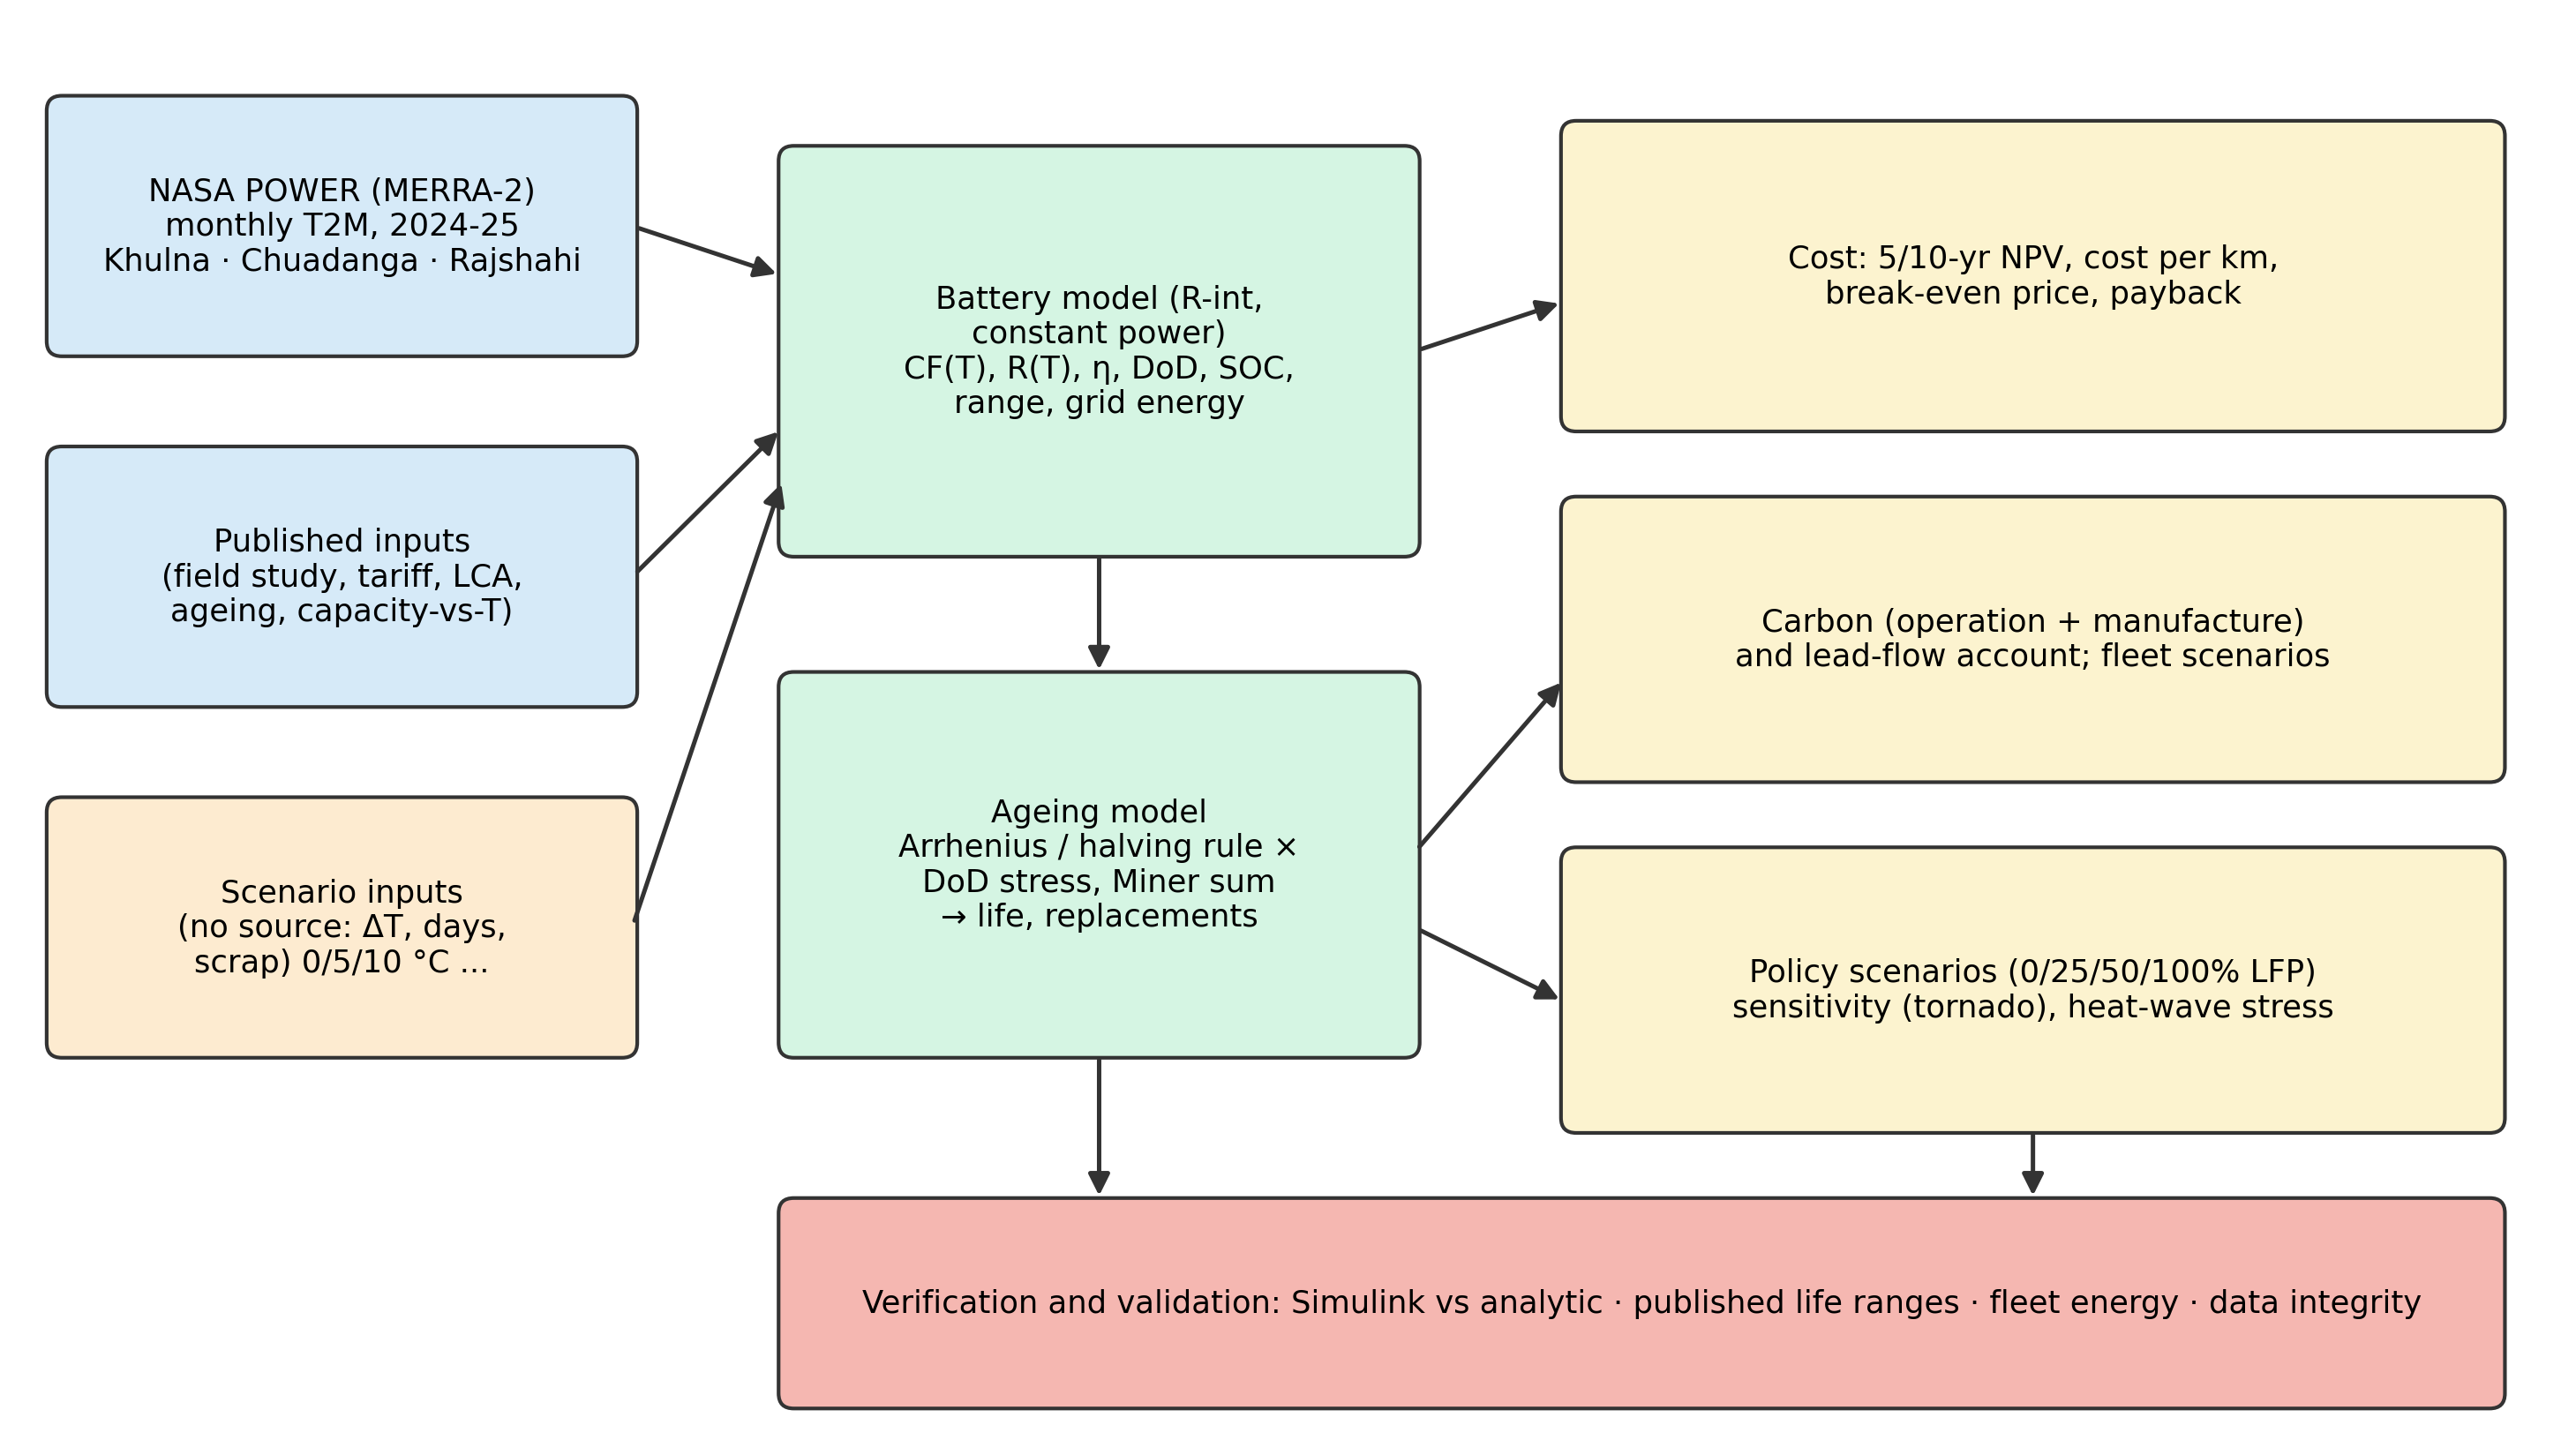
\includegraphics[width=\textwidth]{fig_method.png}\caption{Methodology: temperature and parameter inputs drive the battery and ageing models; outputs feed the cost, carbon, lead and policy modules; verification and validation close the loop.}\label{fig:method}\end{figure}
\subsection{Study design and sites}
Three south-western sites are used: Khulna (22.84$^\circ$N, 89.57$^\circ$E), Chuadanga (23.64$^\circ$N, 88.69$^\circ$E) and Rajshahi (24.38$^\circ$N, 88.60$^\circ$E) (\cref{fig:map}). Chuadanga was selected because a 42$^\circ$C day was reported there in May 2025 \citep{heat2025}, giving a heat-stress case; note that in the NASA monthly means its annual mean (\TannChuadangaBtwofive$^\circ$C in 2025) is not higher than Khulna's (\TannKhulnaBtwofive$^\circ$C), so its selection rests on peak heat, not on the mean. Khulna is also one of the two districts of the field study that supplies the duty-cycle inputs \citep{chowdhury2026}. Three chemistries are compared: lead-acid (LA), LFP and NMC. No operator survey was possible, so every duty-cycle input is taken from published sources or run as a scenario (\cref{tab:params}).
\begin{figure}[t]\centering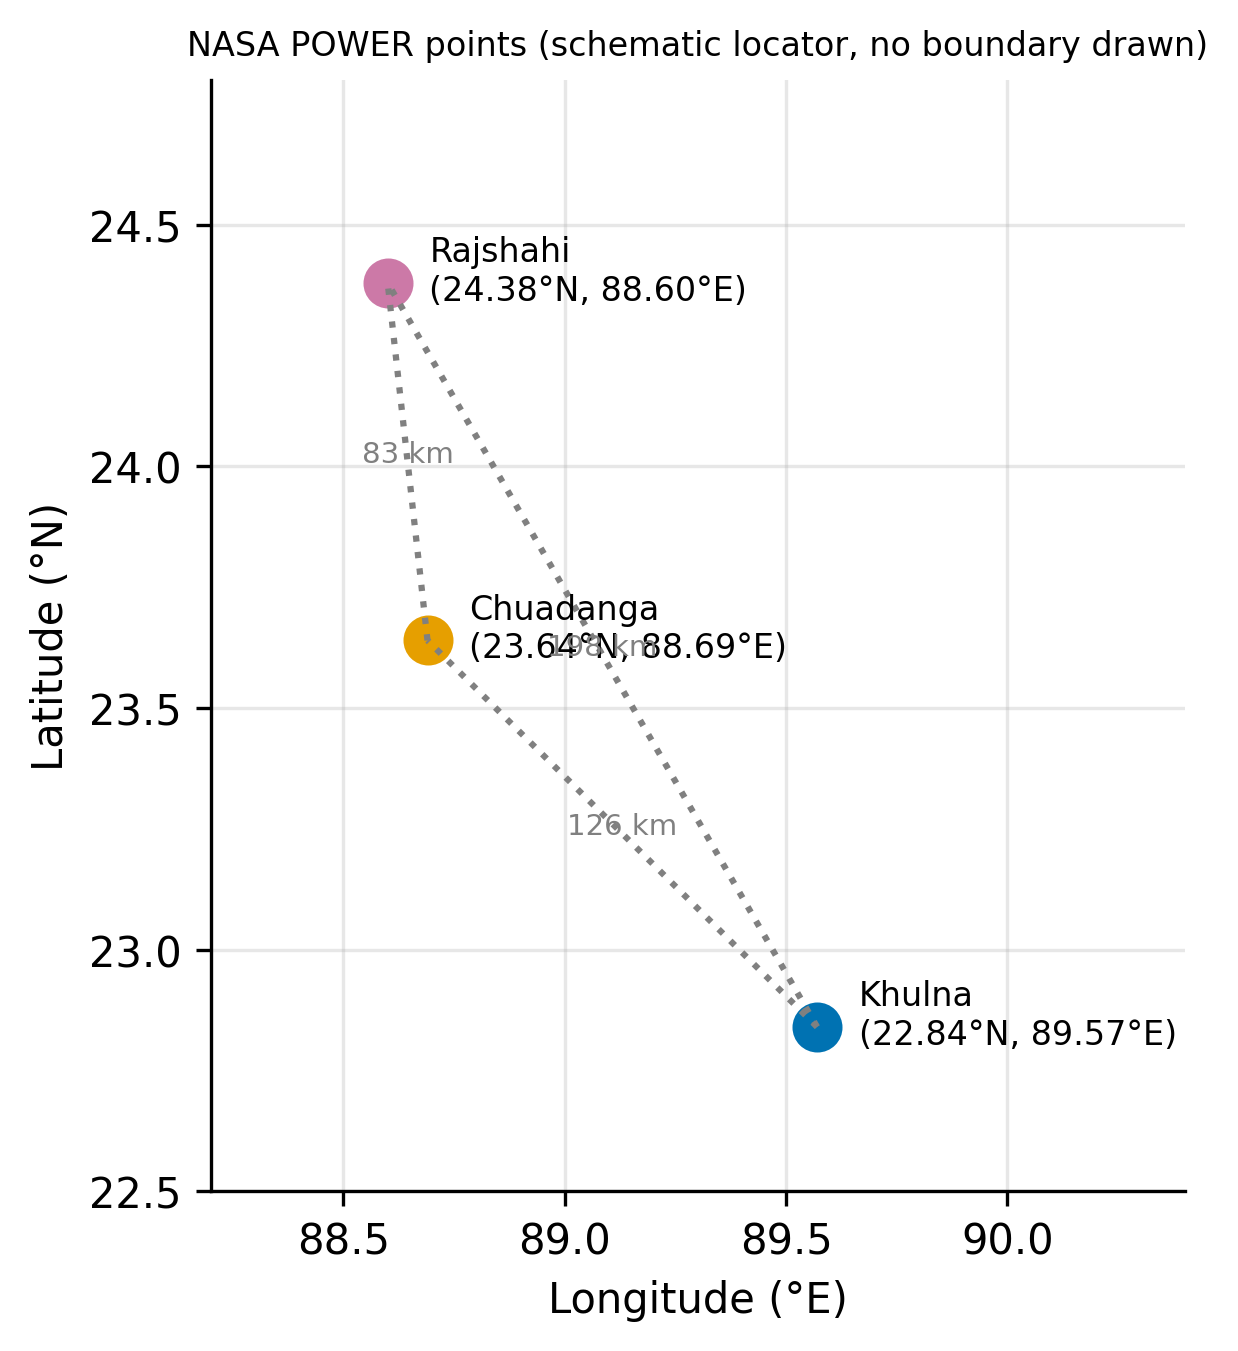
\includegraphics[width=.5\textwidth]{fig_map.png}\caption{NASA POWER grid points used (schematic locator; distances are great-circle).}\label{fig:map}\end{figure}

\subsection{Temperature data}
Monthly mean 2\,m air temperature (T2M, MERRA-2 \citep{gelaro2017}) for January 2024 to December 2025 was downloaded from NASA POWER \citep{nasa_power}: 24 values per site, no missing (-999) entries. The native cell is $0.5^\circ\times0.625^\circ$ (about 50--70~km), so the three points lie in neighbouring cells and are expected to be similar. Battery temperature is ambient plus $\Delta T_{op}=5^\circ$C, a scenario value tested at 0 and 10$^\circ$C. Monthly means understate daily peaks (\cref{sec:limits}).

\subsection{Battery model}
Each pack is a resistive (R-int) battery with temperature-dependent capacity and resistance, discharged at constant average power $P_w=e_{km}v$. With pack voltage $V$ and round-trip efficiency $\eta_{RT}$, the 25$^\circ$C resistance is chosen so that discharge efficiency equals $\sqrt{\eta_{RT}}$ at 25$^\circ$C:
\begin{equation}
R_{25}=\frac{(1-\sqrt{\eta_{RT}})\sqrt{\eta_{RT}}\,V^{2}}{P_w},\quad
R(T)=R_{25}\exp\!\left[\frac{E_r}{R_g}\!\left(\frac1{T_K}-\frac1{298.15}\right)\right],\quad
I=\frac{V-\sqrt{V^{2}-4R(T)P_w}}{2R(T)},\quad
\eta_d=1-\frac{I\,R(T)}{V}.
\end{equation}
The capacity factor $CF(T)$ is interpolated from a table, so the available energy is $E_{cap}=V\,Ah\,CF(T)/1000$~kWh. With daily delivered energy $E_{day}=d\,e_{km}/1000$ for distance $d$:
\begin{align}
DoD&=\frac{E_{day}}{\eta_d\,E_{cap}}, & SOC_{end}&=\max(0,1-DoD),\\
E_{grid}&=\frac{E_{day}}{\eta_d^{2}\,\eta_{chg}}, & \text{Range}&=\frac{DoD_{max}\,E_{cap}\,\eta_d}{e_{km}/1000}.
\end{align}
The same equations are implemented as a Simulink model built from core blocks (\cref{fig:simulink}): constant, lookup tables, product, a function block for the constant-power current, an integrator for SOC, and a sum. It is run at 15, 25, 35 and 45$^\circ$C for all three chemistries and compared with the analytic code (\texttt{easybike\_build\_simulink.m}); the acceptance criterion is 0.5 percentage points in efficiency, 0.01 in end-of-day SOC and 2\% in range. \todo{run easybike\_build\_simulink in MATLAB and report the PASS table here}
\begin{figure}[t]\centering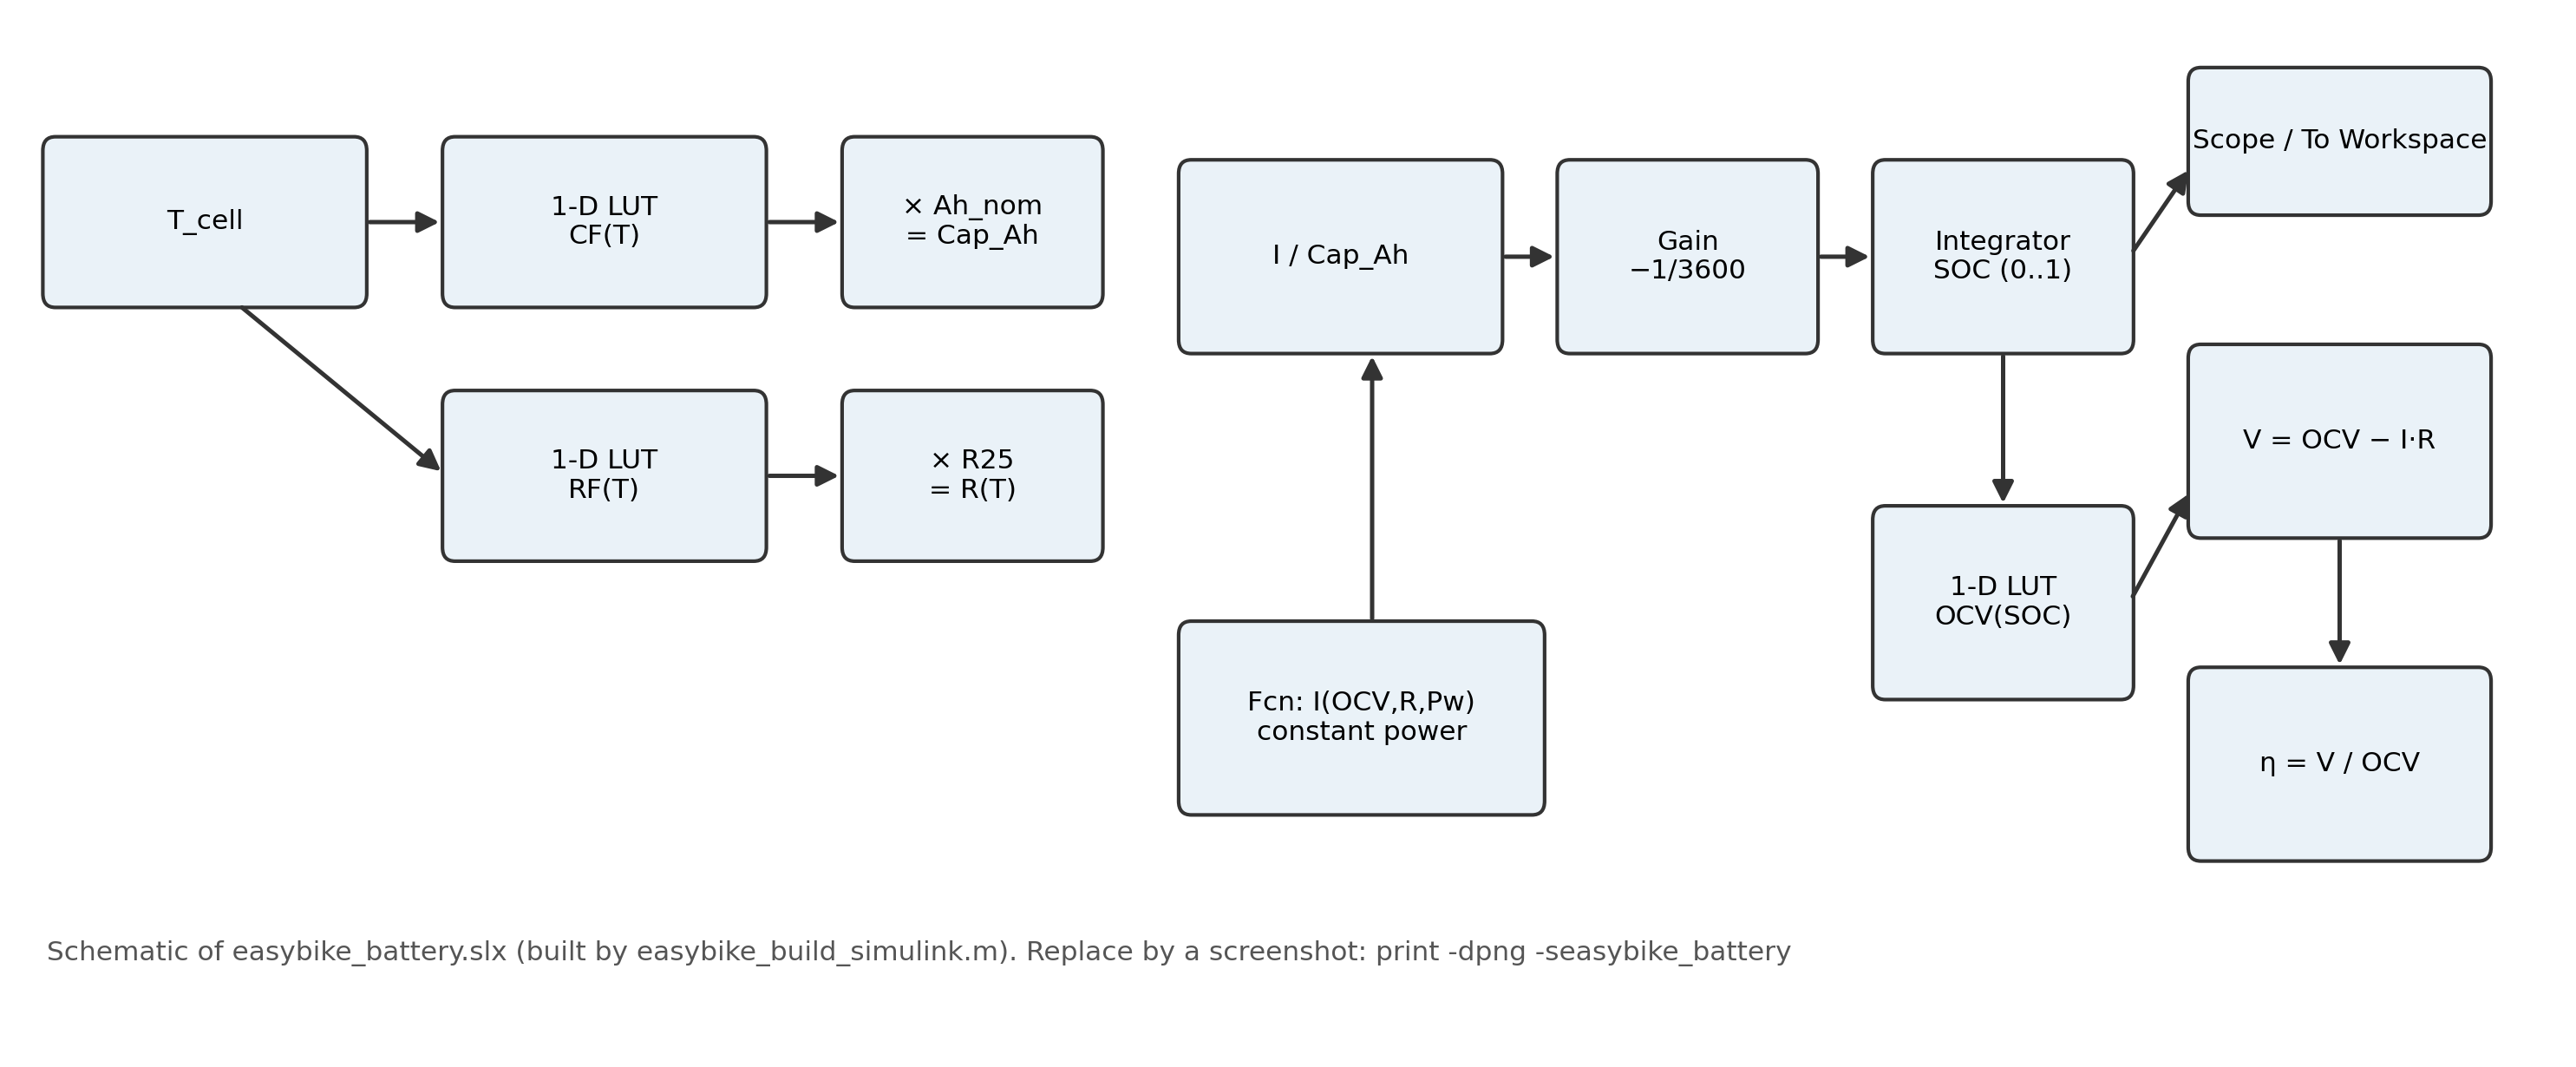
\includegraphics[width=\textwidth]{fig_simulink.png}\caption{Block structure of the Simulink model \texttt{easybike\_battery.slx} (schematic). \todo{optional: replace by a screenshot of the model}}\label{fig:simulink}\end{figure}

\subsection{Degradation and lifetime}
Cycle life falls with depth of discharge and temperature, and damage is accumulated month by month with Miner's rule \citep{miner1945}, as also done for variable-temperature VRLA service \citep{tsujikawa2009}:
\begin{equation}
N_{eff,m}=N_{80}\left(\frac{0.8}{\max(DoD_m,0.05)}\right)^{k} f_T(T_m),\qquad
D=n_{cyc}\sum_m \frac{w_m}{N_{eff,m}},\qquad
L=\frac{1}{D\,d_{op}}\ \text{(years)},
\end{equation}
where $w_m$ is the day-weighted share of month $m$, $d_{op}=300$ operating days per year and $n_{cyc}=1$. For lithium, $f_T=\min\{1,\exp[\tfrac{E_a}{R_g}(\tfrac1{T_K}-\tfrac1{298.15})]\}$ with $E_a=37.3$~kJ/mol (LFP, \citep{yagci2026}) and 10.3~kJ/mol (NMC, derived from \citep{jalkanen2015}); for lead-acid $f_T=\min\{1,2^{-(T-25)/8}\}$ \citep{bu806a}. The cap at 1 gives no life credit below 25$^\circ$C. Calendar ageing is not modelled, so life is cycle-limited (\cref{sec:limits}).

\subsection{Total cost of ownership}
The 5- and 10-year net present cost with discount rate $r$ is
\begin{equation}
TCO_H=C_0+\sum_{j=1}^{K}\frac{C_0(1-s)}{(1+r)^{jL}}-\frac{C_0\,\rho_H}{(1+r)^{H}}+\sum_{t=1}^{H}\frac{E_{grid}\,d_{op}\,\tau + m\,C_0}{(1+r)^t},
\end{equation}
with $C_0$ the pack price, $K=\lfloor H/L\rfloor$ replacements, $s$ the scrap fraction, $\rho_H$ the residual life fraction at horizon $H$, $\tau$ the tariff and $m$ the maintenance fraction. Cost per km is $TCO_{10}$ divided by the discounted distance. The cost is battery-related only (vehicle and driver costs are excluded).

\subsection{Carbon, lead and policy}
Annual emissions per bike are $E_{CO_2}=E_{grid}\,d_{op}\,EF_{grid}+\varepsilon\,Q_{nom}\,12/L_{mo}$ with $EF_{grid}=0.62$~tCO$_2$/MWh \citep{doe_gef}, $Q_{nom}$ the pack energy, $L_{mo}$ the life in months and $\varepsilon=40$, 50, 78.4~kg\,CO$_2$e/kWh (LA, LFP, NMC; \citep{jasper2025,paul2024}). The NMC value is cell-level and the factors come from European studies; Li packs are imported, so LFP is tested up to 110~kg\,CO$_2$e/kWh. A second estimate scales the CLEAN fleet electricity by the modelled LFP-to-LA grid-energy ratio. Informal-smelting emissions have no verified factor and are excluded, which biases the lead-acid footprint downward. Lead cycled per year is $M_{Pb}=N\,m_{Pb}\,12/L_{mo}$ with $m_{Pb}=60$, 90, 125~kg per pack: a mass flow, not an emission or a dose. Policy scenarios move a share $\phi=0$, 25, 50, 100\% of a 1.4~M fleet from LA to LFP; outputs scale linearly.

\subsection{Validation and sensitivity}
Five checks are made: V1 data integrity; V2 energy use against published values (a 110~km-per-charge benchmark of five 120~Ah batteries \citep{techno2016} and 71.4--88~Wh/km \citep{peakdemand}); V3 modelled life against reported ranges (8--12 months for lead-acid \citep{fe2024}; 60--84 and 36--48 months for LFP and NMC from the data file); V4 grid energy against the 8--9~kWh per charge of the field study \citep{chowdhury2026} (used for calibration, so not independent) and against the CLEAN fleet figure (independent); V5 Simulink against the analytic model. One-at-a-time sensitivity (11 inputs, \cref{fig:tornado}) and scenario runs for battery temperature, distance, scrap value and tariff address inputs without a published source.

\section{Results}
\subsection{Temperature input}
Monthly mean T2M follows the same seasonal cycle at all three sites, from about \Tmin$^\circ$C in January to \Tmax$^\circ$C in April 2024 (\cref{fig:temp}). Mean battery temperature is \TcKhulna, \TcChuadanga{} and \TcRajshahi$^\circ$C at Khulna, Chuadanga and Rajshahi, a spread of \Tspread$^\circ$C (\cref{tab:results}).
\begin{figure}[t]\centering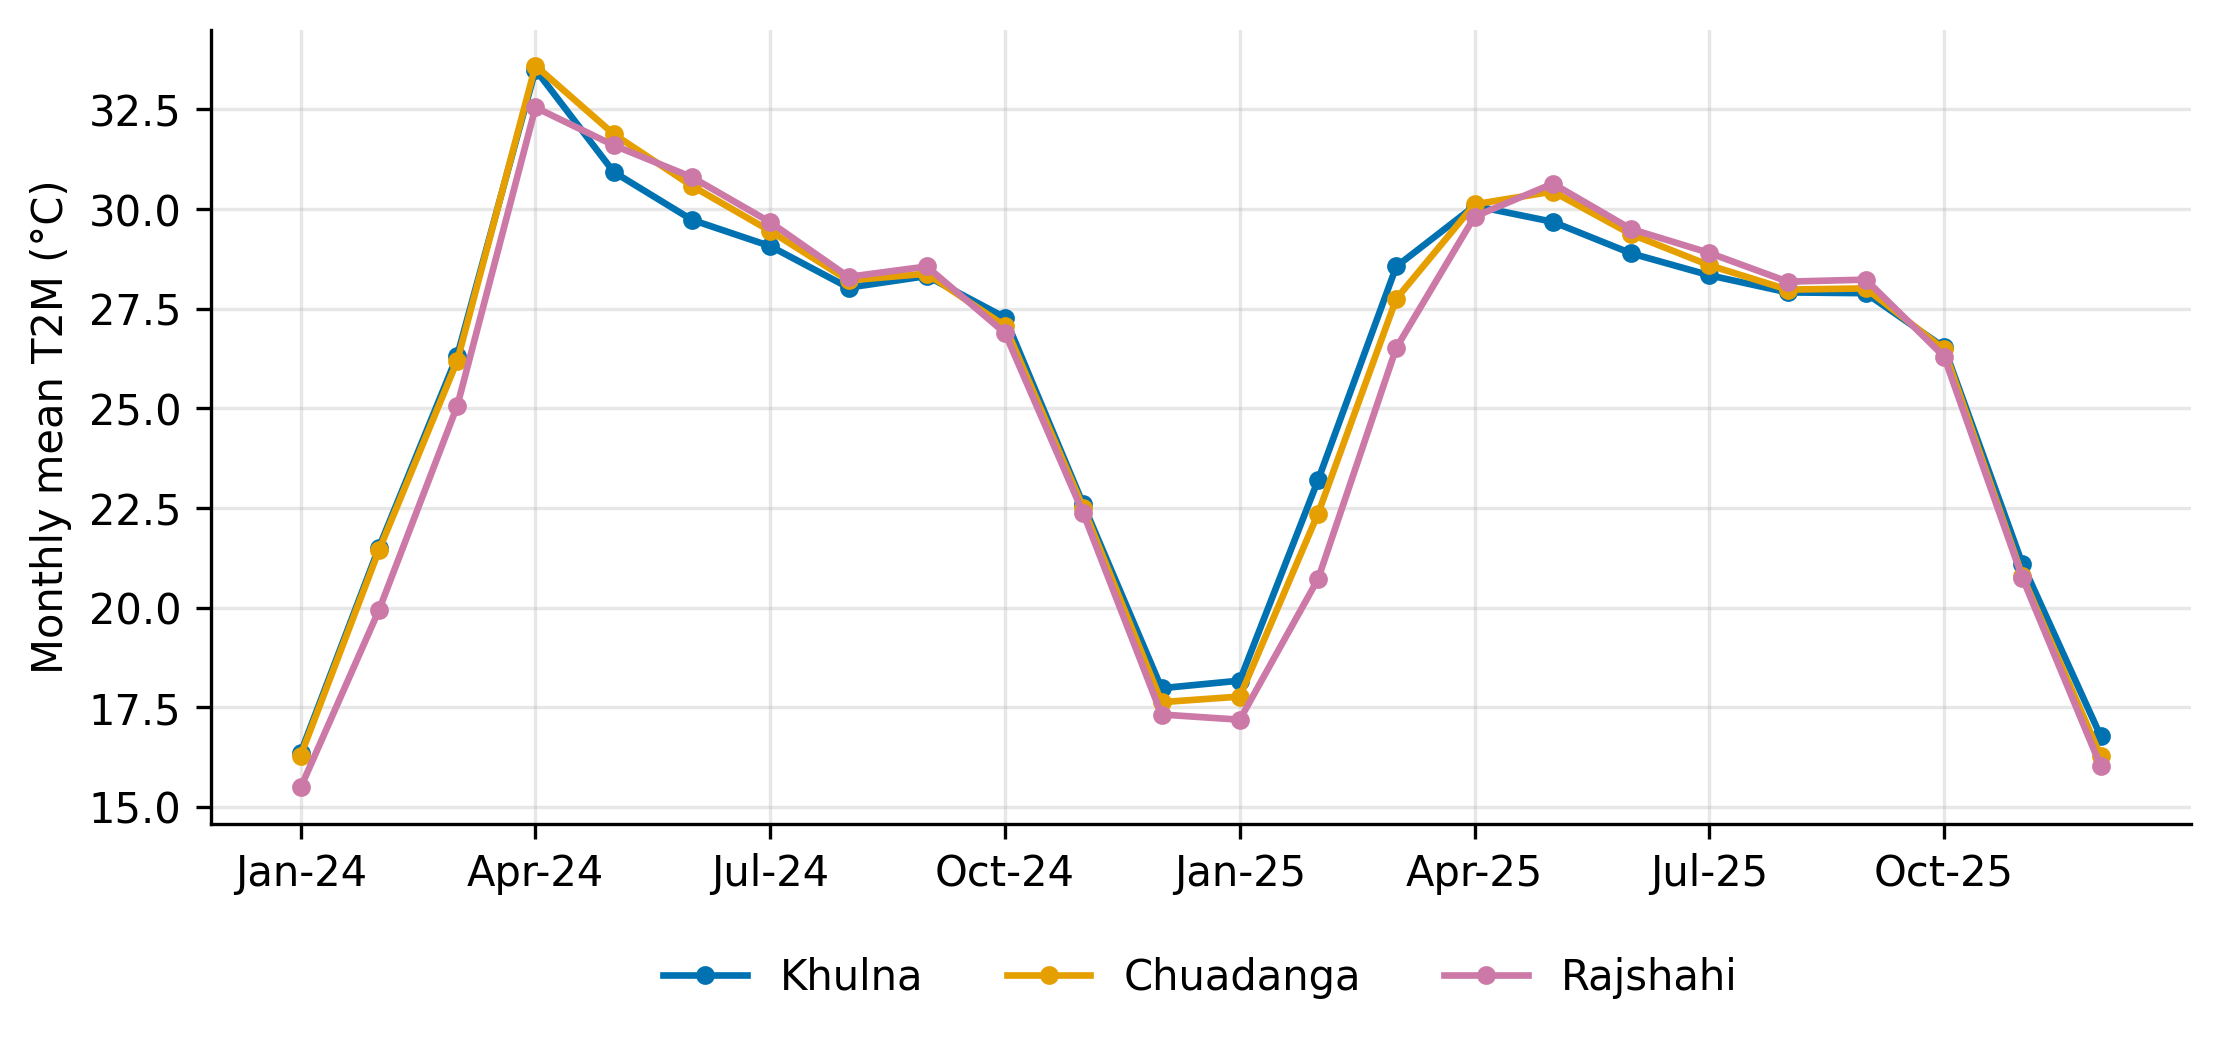
\includegraphics[width=.8\textwidth]{fig1_temperature.png}\caption{NASA POWER monthly mean 2\,m temperature at the three sites, Jan 2024--Dec 2025.}\label{fig:temp}\end{figure}

\subsection{Performance, life and cost}
\begin{table*}[t]
\centering\small
\caption{Simulated 24-month results (NASA POWER monthly $T_{2m}$, Jan 2024--Dec 2025; battery temperature = ambient + 5~$^\circ$C). Source: \texttt{results\_summary.csv} from \texttt{easybike\_main.m}. Life is in months of operation at 300~days\,yr$^{-1}$; TCO is net present value at an 11.57\% discount rate and a tariff of BDT 11.36/kWh.}
\label{tab:results}
\begin{tabular}{llrrrrrrrrr}
\toprule
Site & Battery & $\bar T_{cell}$ & $\eta$ & DoD & Range & $E_{grid}$ & Life & Repl. & TCO$_{10}$ & Cost \\
 & & ($^\circ$C) & (\%) & (\%) & (km) & (kWh/d) & (mo) & (10~yr) & ($10^3$ BDT) & (BDT/km) \\
\midrule
Khulna & Lead-Acid & 30.8 & 90.2 & 63.5 & 83.3 & 8.10 & 12.4 & 9 & 725 & 6.37 \\
 & LFP & 30.8 & 97.8 & 69.4 & 76.1 & 6.87 & 83.7 & 1 & 342 & 3.00 \\
 & NMC & 30.8 & 96.7 & 69.5 & 76.0 & 7.03 & 52.9 & 2 & 437 & 3.84 \\
\midrule
Chuadanga & Lead-Acid & 30.8 & 90.2 & 63.5 & 83.3 & 8.10 & 12.2 & 9 & 731 & 6.42 \\
 & LFP & 30.8 & 97.8 & 69.4 & 76.1 & 6.87 & 83.2 & 1 & 342 & 3.01 \\
 & NMC & 30.8 & 96.7 & 69.5 & 76.0 & 7.03 & 52.8 & 2 & 437 & 3.84 \\
\midrule
Rajshahi & Lead-Acid & 30.5 & 90.0 & 63.7 & 83.0 & 8.13 & 12.4 & 9 & 724 & 6.36 \\
 & LFP & 30.5 & 97.8 & 69.5 & 76.0 & 6.88 & 84.0 & 1 & 341 & 2.99 \\
 & NMC & 30.5 & 96.7 & 69.6 & 75.9 & 7.04 & 52.9 & 2 & 437 & 3.84 \\
\bottomrule
\end{tabular}
\end{table*}

\Cref{tab:results,fig:comp} give the main comparison. Discharge efficiency is about \effLA\% (LA), \effLFP\% (LFP) and \effNMC\% (NMC). Modelled life is \lifeLA{} months for LA, \lifeNMC{} for NMC and \lifeLFP{} for LFP (site mean), i.e.\ about \repLA{} LA packs but \repLFP{} LFP pack replacement in ten years. The 10-year net present cost per bike is BDT \tcoLA{} (LA), \tcoNMC{} (NMC) and \tcoLFP{} (LFP): LFP saves BDT \tcoSave{} per bike, and its cost per km (\cpkLFP\ BDT) is less than half that of LA (\cpkLA\ BDT). The LA bank has the longest range (\rngLA{} vs \rngLFP~km) because it stores more energy (9.0 vs 7.7~kWh), not because it is more efficient. All packs run close to the 80\% DoD limit in some months (maximum \dodmaxLA/\dodmaxLFP/\dodmaxNMC\%), which is realistic for easy-bike duty.
\begin{figure}[t]\centering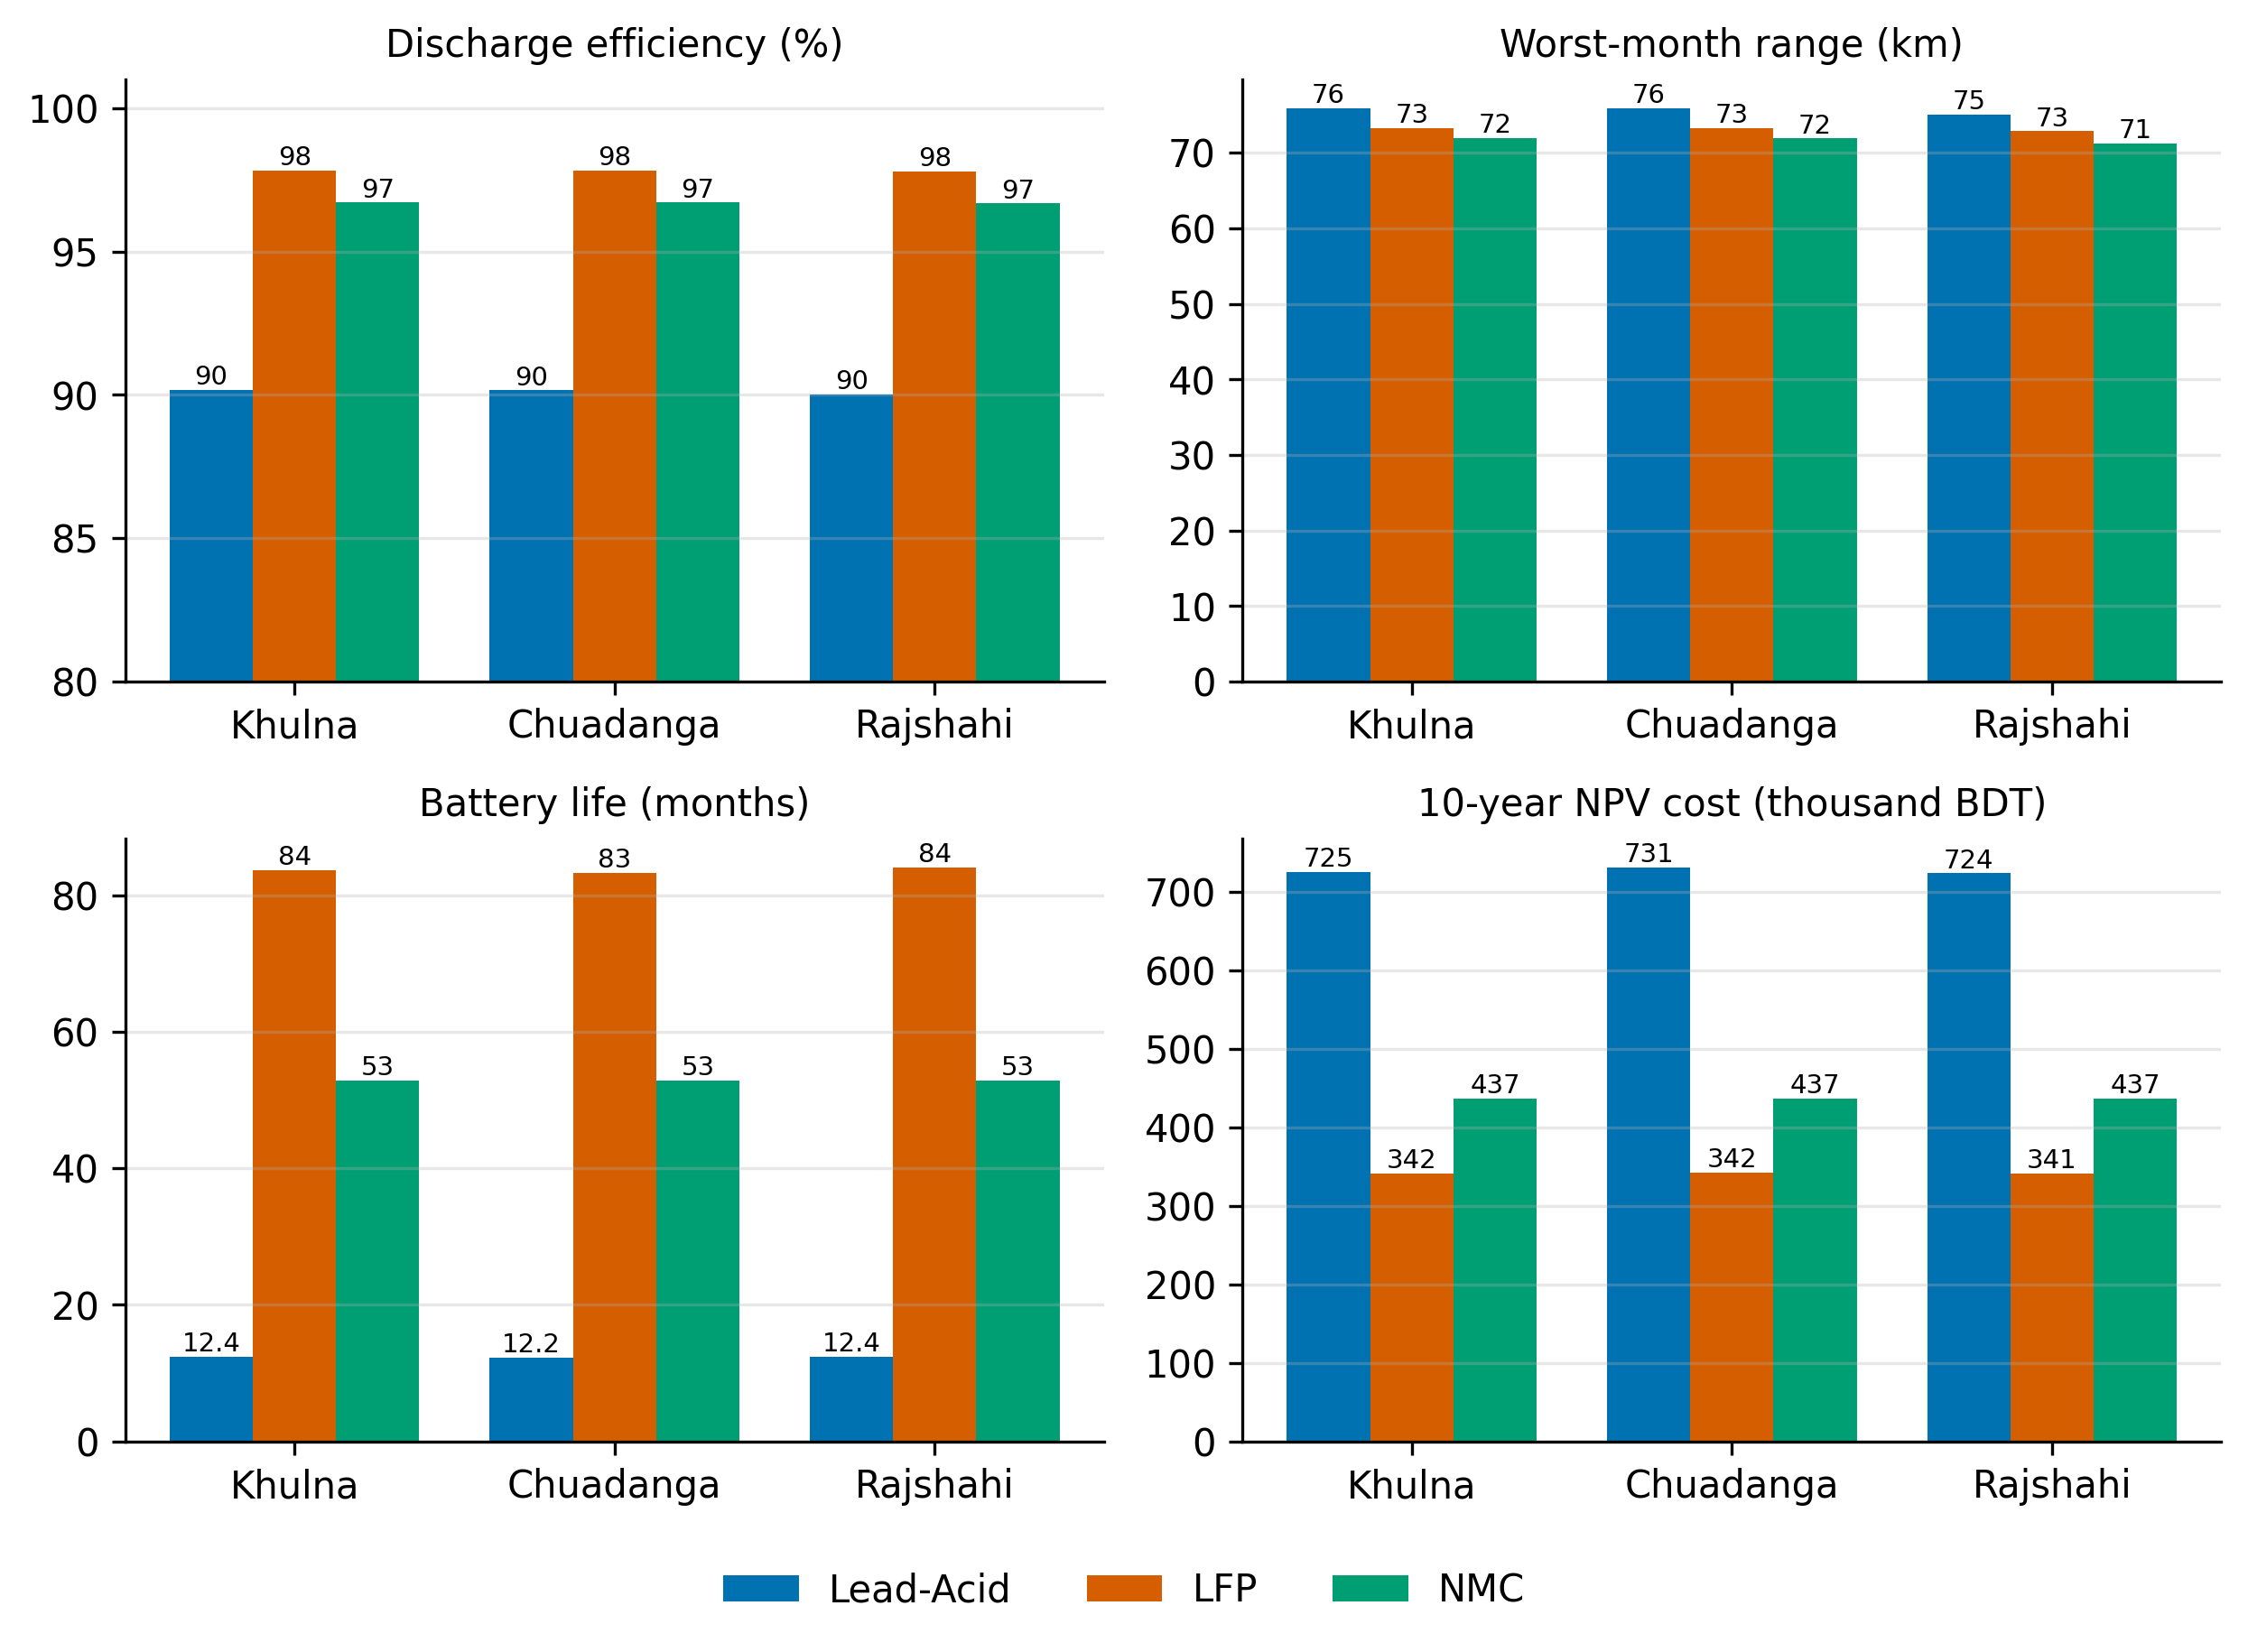
\includegraphics[width=.9\textwidth]{fig2_comparison.png}\caption{Site comparison of discharge efficiency, worst-month range, battery life and 10-year NPV cost.}\label{fig:comp}\end{figure}
\begin{figure}[t]\centering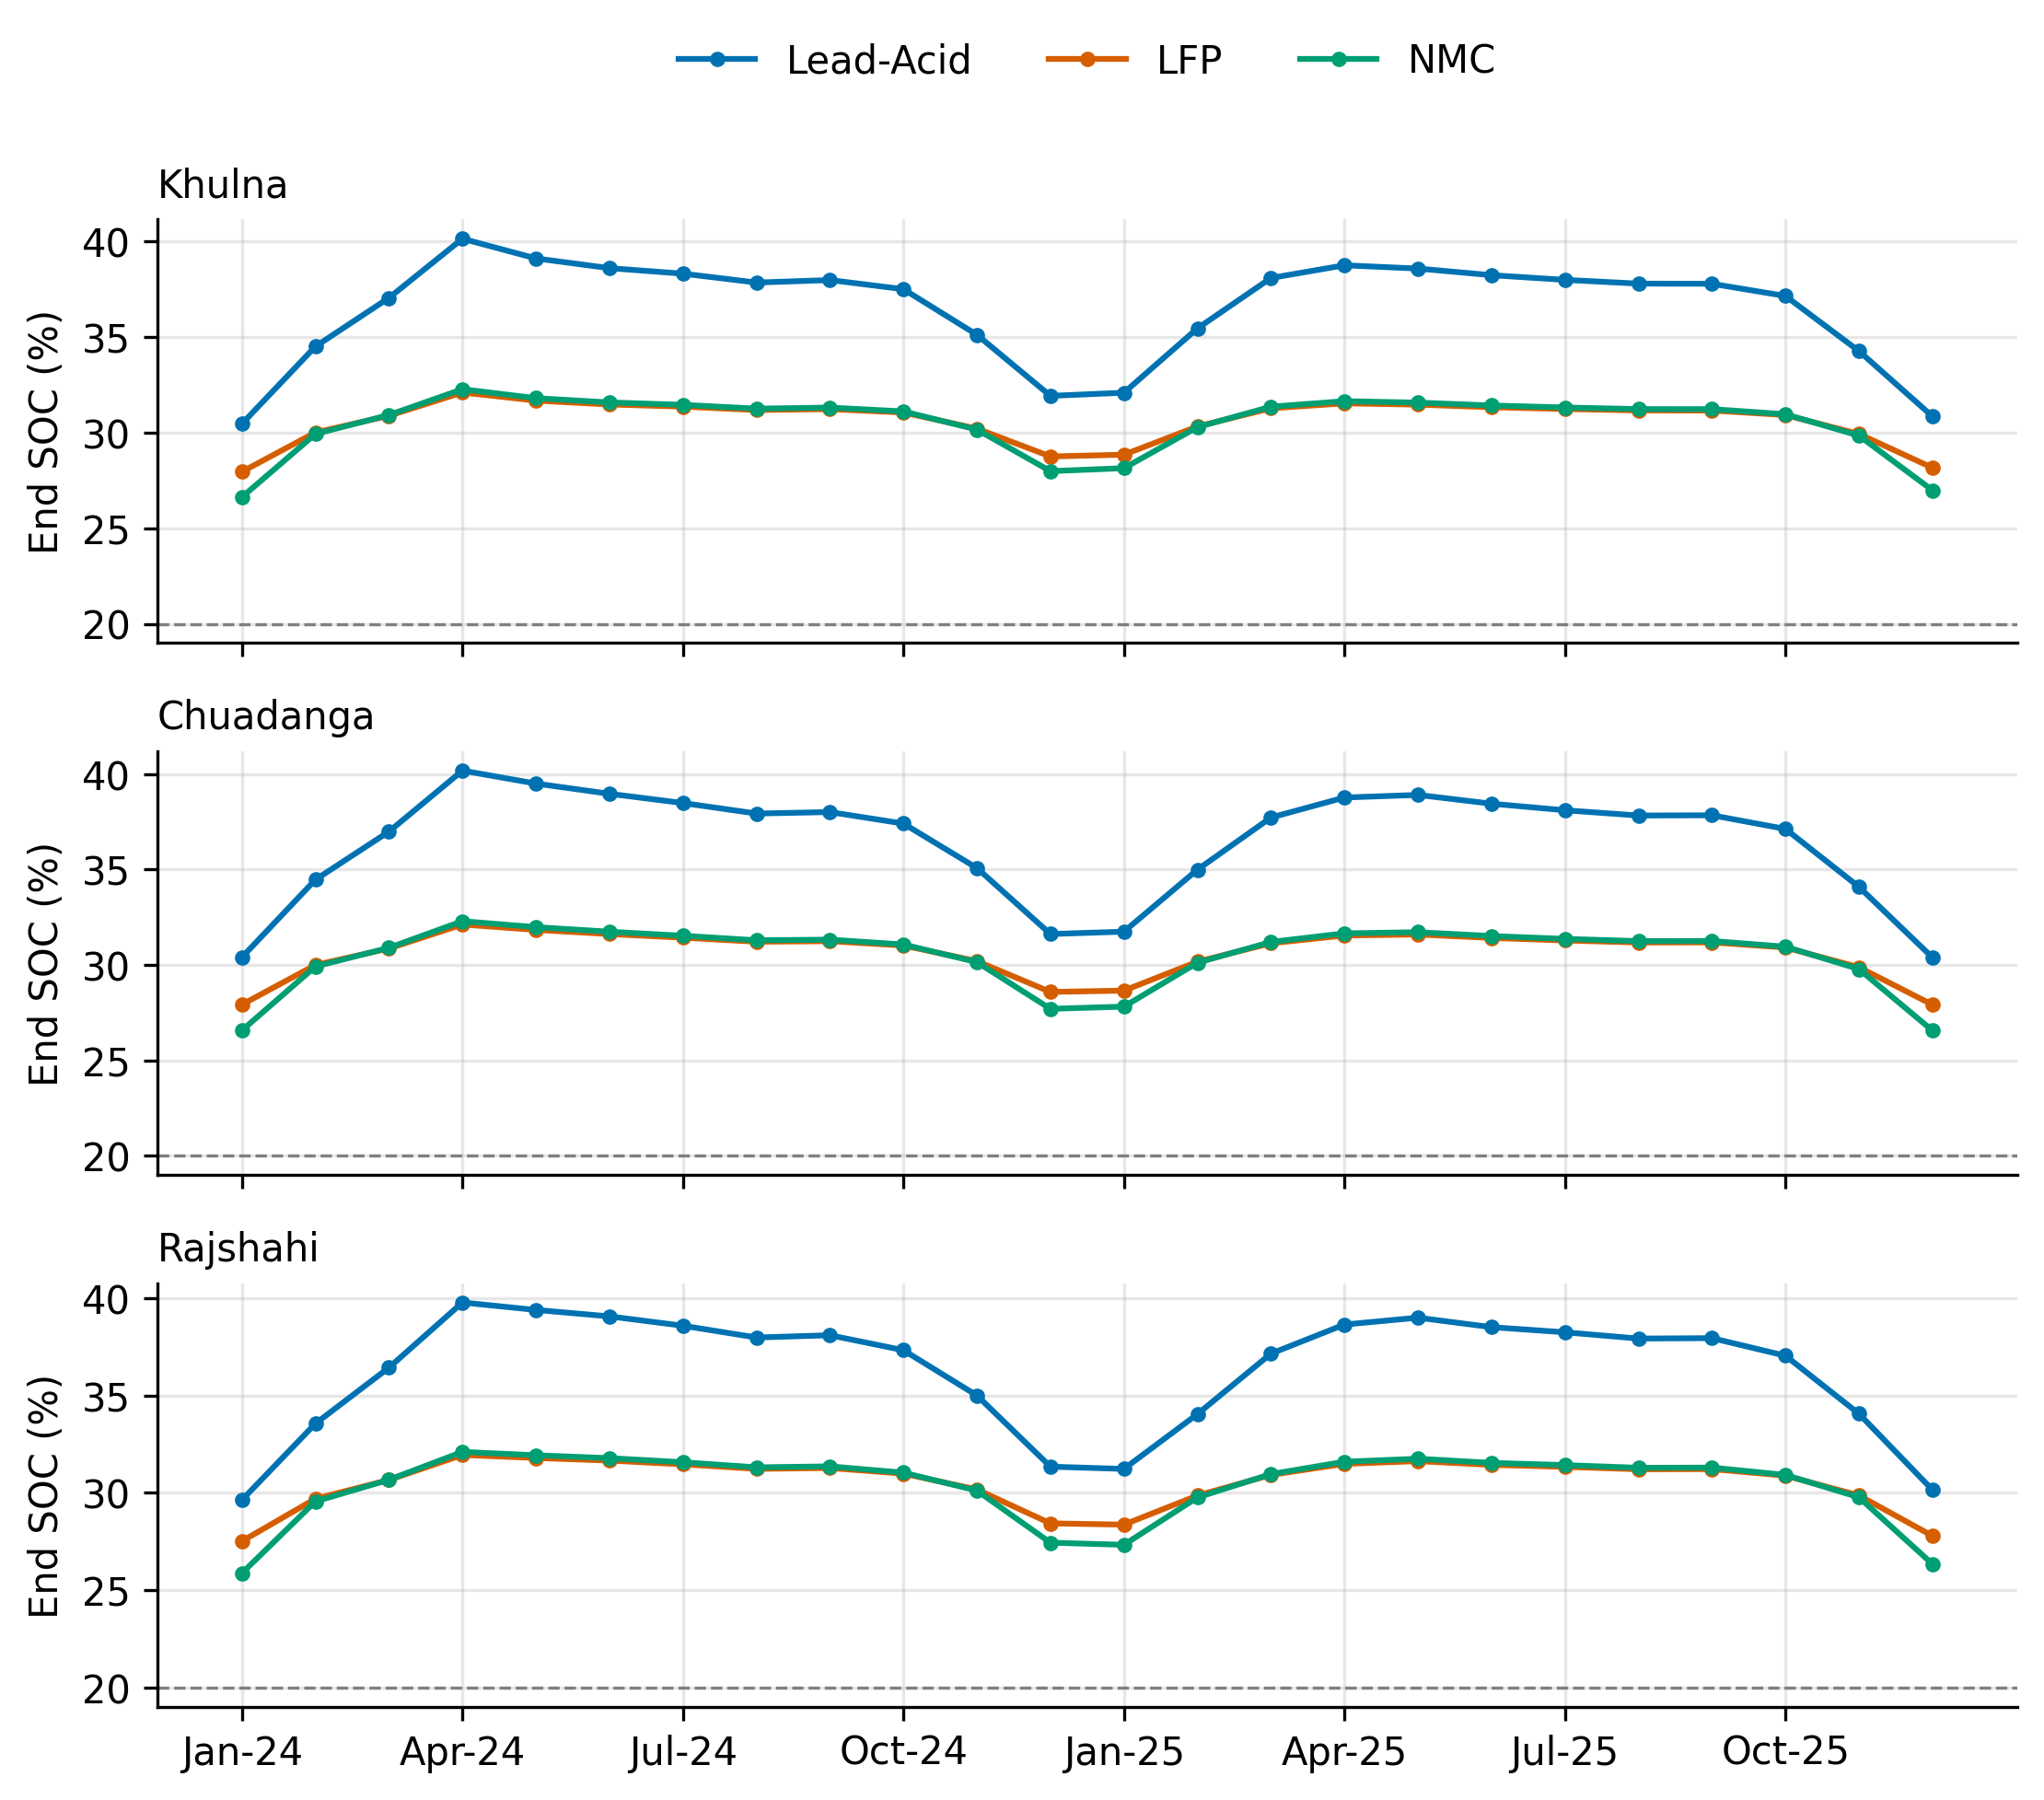
\includegraphics[width=.85\textwidth]{fig3_soc.png}\caption{Month-end state of charge after one day's discharge; dashed line = 20\% limit.}\label{fig:soc}\end{figure}

\subsection{Heat-wave stress}
At 42$^\circ$C ambient (Chuadanga, 10 May 2025 \citep{heat2025}) with the 5$^\circ$C offset, LA ages \heatLA{} times, LFP \heatLFP{} times and NMC \heatNMC{} times faster than in the 2024--25 monthly-mean climate. The absolute life gap between lead-acid and lithium therefore widens in heat.

\subsection{Scenarios, sensitivity and break-even}\label{sec:sens}
\begin{table}[t]
\centering\small
\caption{Scenario runs for inputs without a published source. Upper block: battery temperature rise above ambient (site mean). Lower block: daily distance at Chuadanga (max DoD $>$100\% means the pack cannot serve the duty).}
\label{tab:scen}
\begin{tabular}{lrrrrrr}
\toprule
 & \multicolumn{3}{c}{Life (months)} & \multicolumn{3}{c}{10-yr TCO (10$^3$ BDT)} \\
 & LA & LFP & NMC & LA & LFP & NMC \\
\midrule
$\Delta T$ = +0 $^\circ$C & 16.3 & 98.9 & 54.0 & 604 & 321 & 433 \\
$\Delta T$ = +5 $^\circ$C & 12.4 & 83.6 & 52.9 & 727 & 342 & 437 \\
$\Delta T$ = +10 $^\circ$C & 8.7 & 68.1 & 50.7 & 950 & 370 & 446 \\
\midrule
40 km/day (max DoD 42/44/45\%) & 24.7 & 137.3 & 87.1 & 397 & 237 & 295 \\
60 km/day (max DoD 63/66/67\%) & 14.0 & 91.5 & 58.1 & 649 & 317 & 402 \\
66 km/day (max DoD 70/72/73\%) & 12.2 & 83.2 & 52.8 & 731 & 342 & 437 \\
80 km/day (max DoD 84/87/89\%) & 9.4 & 68.7 & 43.6 & 932 & 398 & 515 \\
100 km/day (max DoD 105/109/111\%) & 6.8 & 54.9 & 34.9 & 1240 & 480 & 627 \\
\bottomrule
\end{tabular}
\end{table}

\Cref{tab:scen} shows that the battery temperature rise and daily distance change life and cost strongly. A battery 10$^\circ$C above ambient cuts LA life to 8.7 months, while 0$^\circ$C raises it to 16.3. At 100~km per day none of the three packs can serve the duty within 100\% DoD, and at 40~km per day all last far longer. The tornado chart (\cref{fig:tornado}) ranks daily distance, battery temperature rise and energy use above price, tariff or ageing parameters. LFP stays cheaper than LA up to an LFP pack price of BDT \beLFP{} (model price \priceLFP), BDT \beDistLow{} at 40~km per day and BDT \beTten{} at +10$^\circ$C. The up-front premium of BDT \premium{} is repaid in about \paybackYr{} year of running savings (undiscounted).
\begin{figure}[t]\centering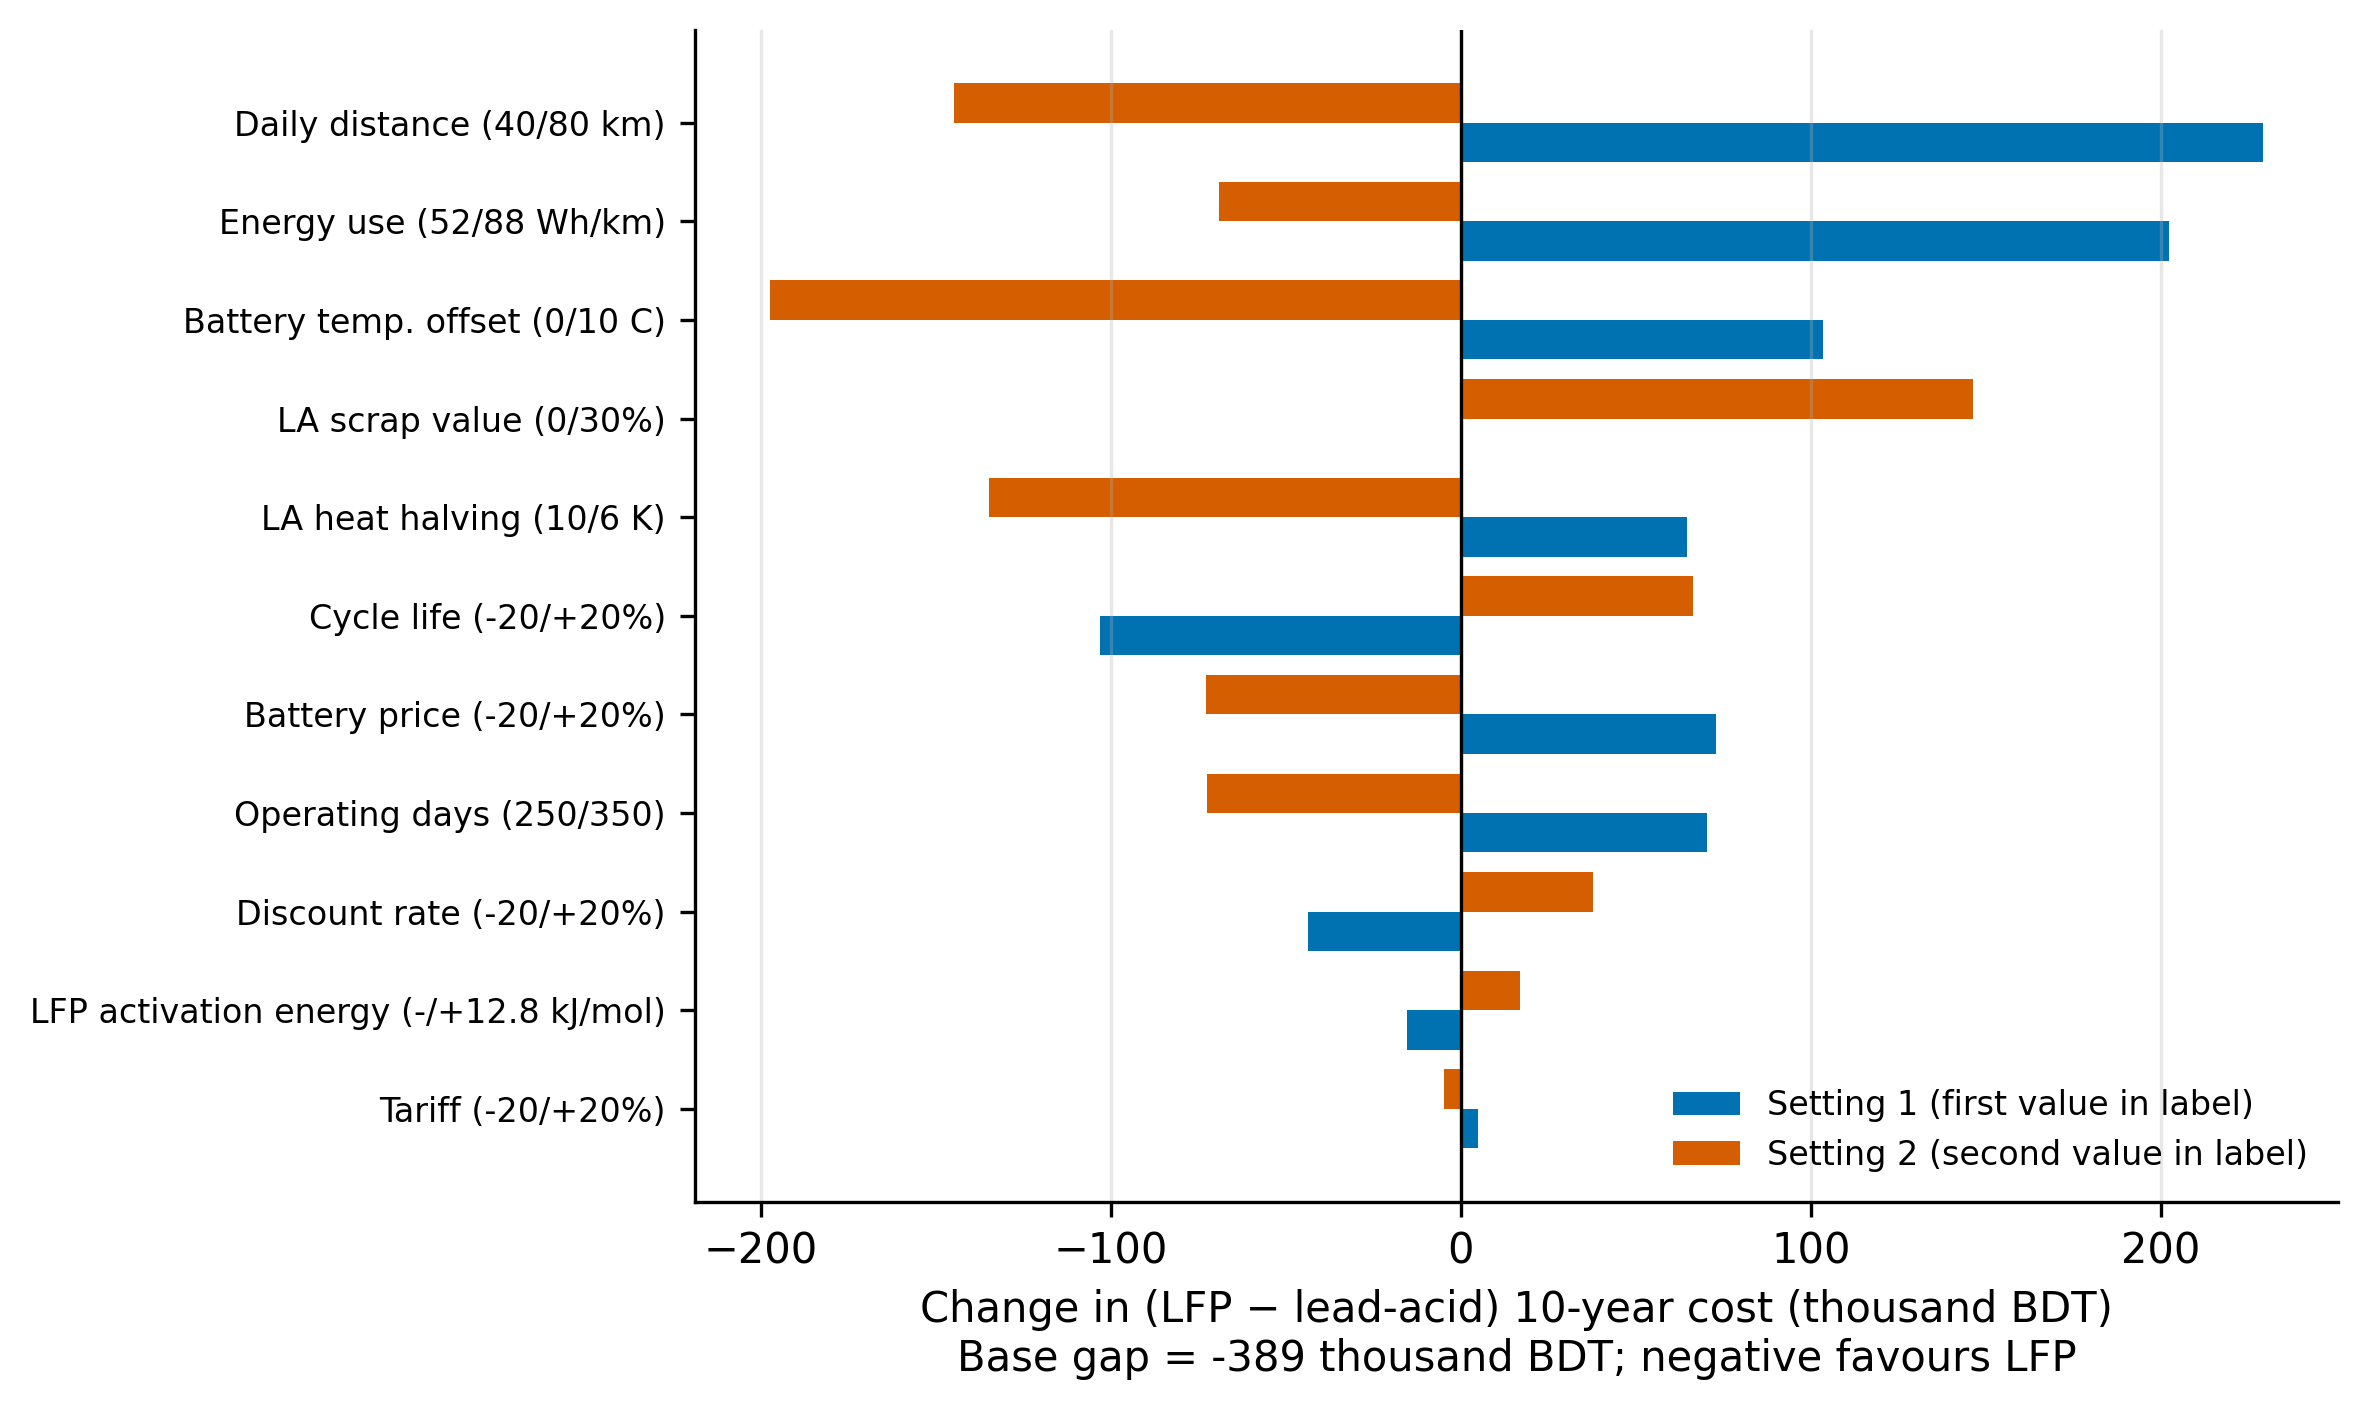
\includegraphics[width=.85\textwidth]{fig4_tornado.png}\caption{One-at-a-time sensitivity of the LFP-minus-LA 10-year cost gap at Chuadanga (base gap $-$\gapBase\ BDT). Negative values favour LFP.}\label{fig:tornado}\end{figure}
\paragraph{When does LFP stop being cheaper?} We combined the settings most unfavourable to LFP: 40~km per day, no battery heating, LA scrap value 30\% of price, LA halving every 10~K, and an LFP price 20\% above the model value. LFP is still cheaper by BDT \jointGap{}. If the LFP price is 50\% higher in that same case, LA becomes cheaper by BDT \jointGapHigh. LFP's cost advantage is therefore robust to any single assumption but not to a combination of several, and the LA scrap value is the most important missing datum (\cref{tab:scen} and the tornado: a 30\% scrap value cuts the gap by BDT \scrapThirty).

\subsection{Validation}
V1 passed (24 months per site, no gaps). V2 passed: 79.7~Wh/km lies inside the 52--88~Wh/km spanned by the published values. V3 (\cref{fig:valid}): LFP life (\lifeLFP~mo) lies at the upper edge of the 60--84 reported; LA life (\lifeLA~mo) is \vLApct\% above the 8--12 months field range; NMC life (\lifeNMC~mo) is \vNMCpct\% above 36--48. V4: modelled lead-acid grid energy (\vEgrid~kWh per bike-day) is \vCleanPct\% below the CLEAN-implied \vClean~kWh, a gap that only field metering can resolve (the CLEAN figure may include other vehicle types and charging losses). V5 is the Simulink cross-check described in the Methodology. The model is therefore plausible against the published ranges but is \emph{not} validated against operator records.
\begin{figure}[t]\centering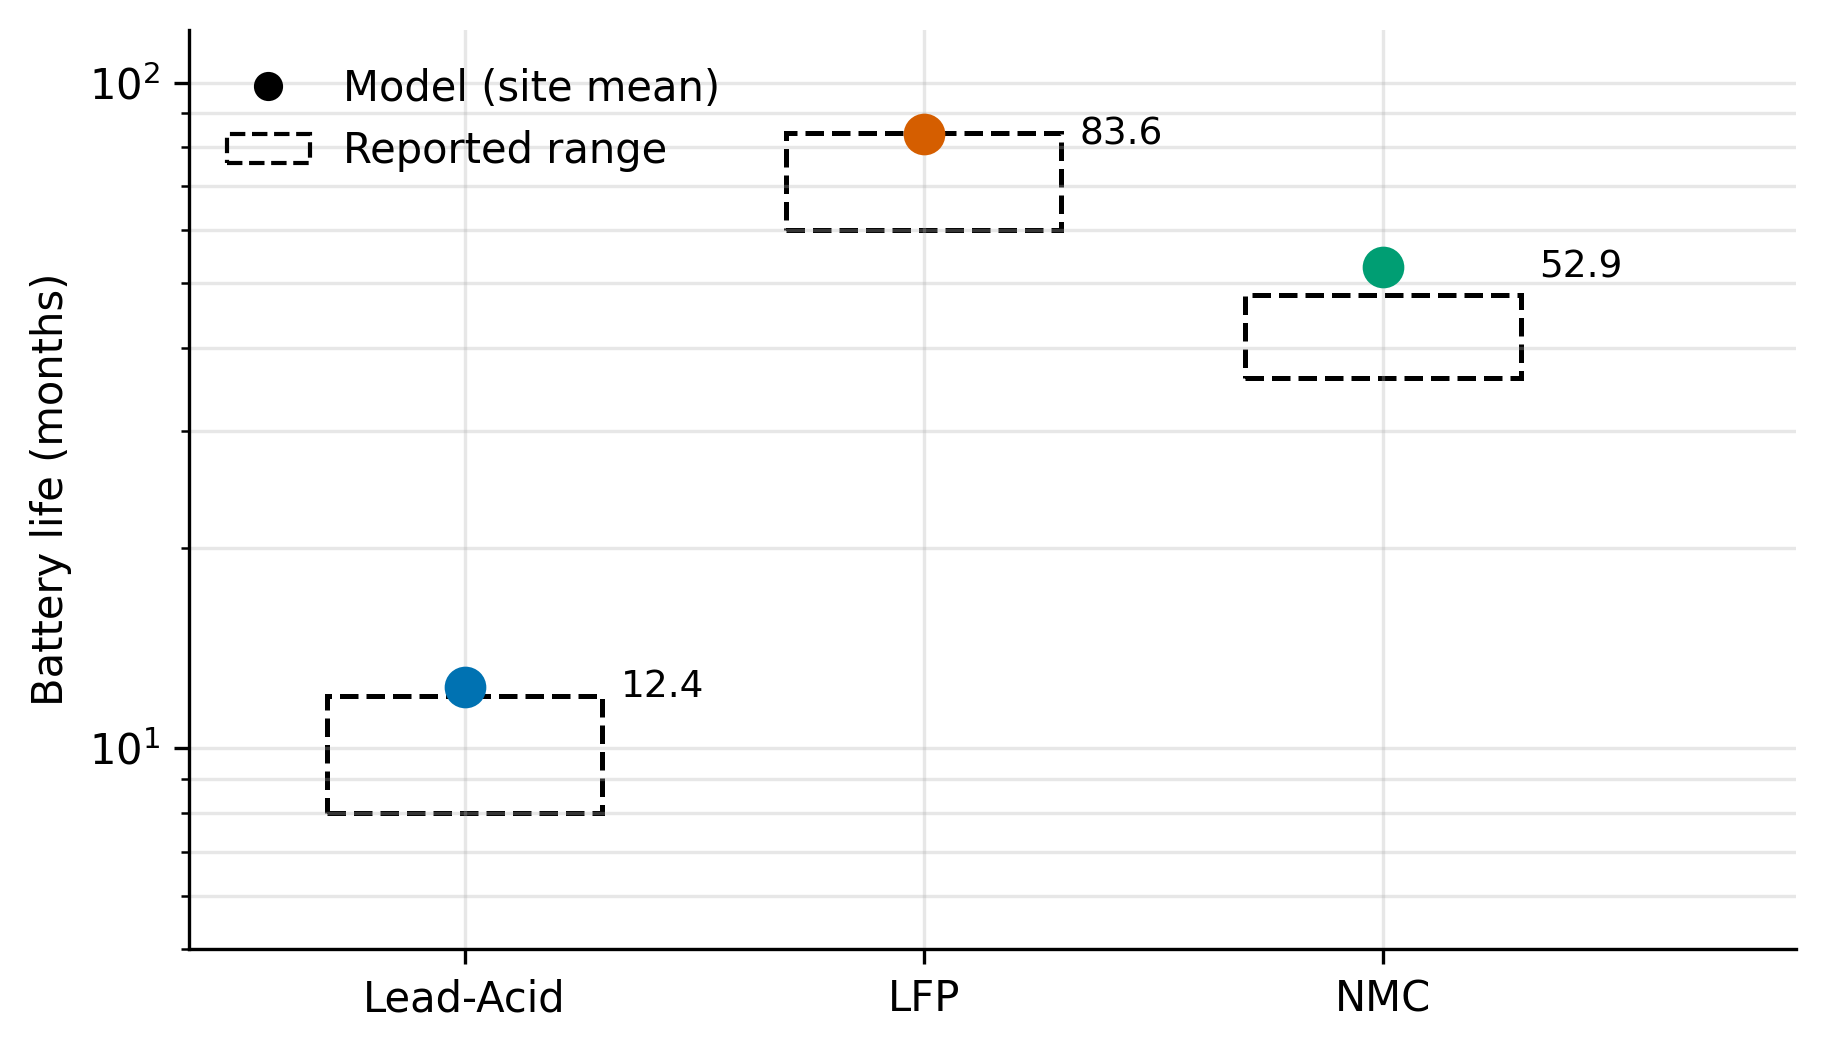
\includegraphics[width=.6\textwidth]{fig_valid.png}\caption{Modelled battery life (site mean) against reported ranges (dashed boxes; logarithmic axis).}\label{fig:valid}\end{figure}

\subsection{Carbon footprint}
\begin{table}[t]
\centering\small
\caption{Carbon budget per bike per year (site-averaged; grid factor 0.62~tCO$_2$/MWh; manufacture+end-of-life factors per kWh of pack capacity: 40 (lead-acid), 50 (LFP), 78.4 (NMC) kg\,CO$_2$e).}
\label{tab:co2bike}
\begin{tabular}{lrrrr}
\toprule
Battery & Packs/yr & Operation & Manufacture+EOL & Total \\
 & (--) & (kg CO$_2$e) & (kg CO$_2$e) & (kg CO$_2$e) \\
\midrule
Lead-acid & 0.97 & 1508 & 350 & 1858 \\
LFP & 0.14 & 1279 & 55 & 1334 \\
NMC & 0.23 & 1308 & 138 & 1447 \\
\bottomrule
\end{tabular}
\end{table}

A lead-acid easy-bike causes about \perbikeLA{}~kg\,CO$_2$e per year, an LFP bike \perbikeLFP{} and an NMC bike \perbikeNMC{} (\cref{tab:co2bike,fig:co2}). Switching one bike to LFP saves \saveLFPbike{}~kg\,CO$_2$e per year, \saveLFPop{} from lower electricity use and \saveLFPemb{} from fewer manufactured packs (\packsLA{} LA packs against \packsLFP{} LFP packs per year). For 1.4~M bikes this is \fleetLFPa{}~Mt\,CO$_2$e per year, or \fleetLFPb{}~Mt for 3~M bikes (\cref{tab:co2fleet}). The independent CLEAN-based estimate, electricity only, gives \cleanGWh{}~GWh and \cleanMt{}~Mt\,CO$_2$ per year. The per-bike saving stays between \sensMin{} and \sensMax{}~kg per year for LFP manufacturing between 50 and 110~kg\,CO$_2$e/kWh and grid factors of 0.55--0.70 (\cref{fig:co2sens}).
\begin{figure}[t]\centering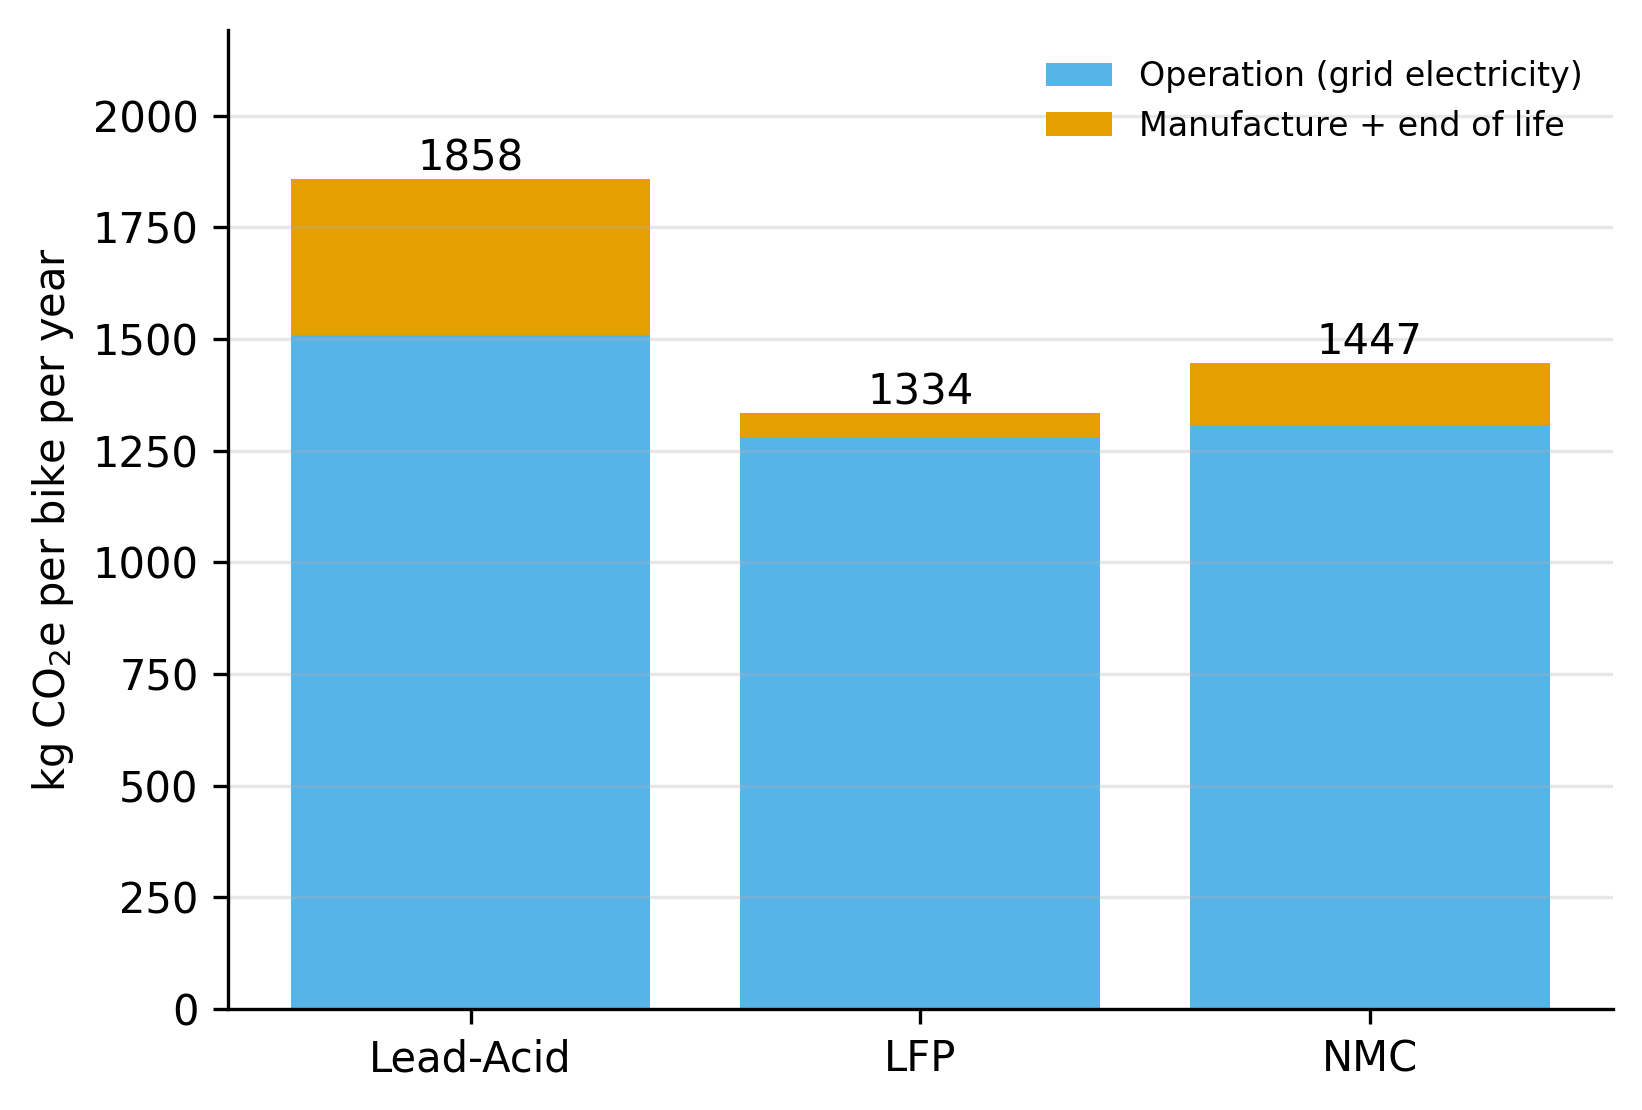
\includegraphics[width=.62\textwidth]{fig5_co2_bike.png}\caption{Annual carbon footprint per bike, split into operation and manufacture+end-of-life.}\label{fig:co2}\end{figure}
\begin{table}[t]
\centering\small
\caption{Fleet-level annual CO$_2$e under two fleet-size scenarios; savings are lead-acid minus the alternative if the \emph{entire} fleet switched.}
\label{tab:co2fleet}
\begin{tabular}{lrr}
\toprule
 & 1.4 M bikes \citep{clean2024} & 3.0 M bikes (lower bound of 3--4 M \citep{pureearth_smep}) \\
 & (Mt CO$_2$e/yr) & (Mt CO$_2$e/yr) \\
\midrule
Lead-acid fleet (baseline) & 2.60 & 5.57 \\
Saving, all LFP (operation) & 0.32 & 0.69 \\
Saving, all LFP (manufacture+EOL) & 0.41 & 0.88 \\
\textbf{Saving, all LFP (total)} & \textbf{0.73} & \textbf{1.57} \\
Saving, all NMC (total) & 0.58 & 1.23 \\
\bottomrule
\end{tabular}
\end{table}

\begin{figure}[t]\centering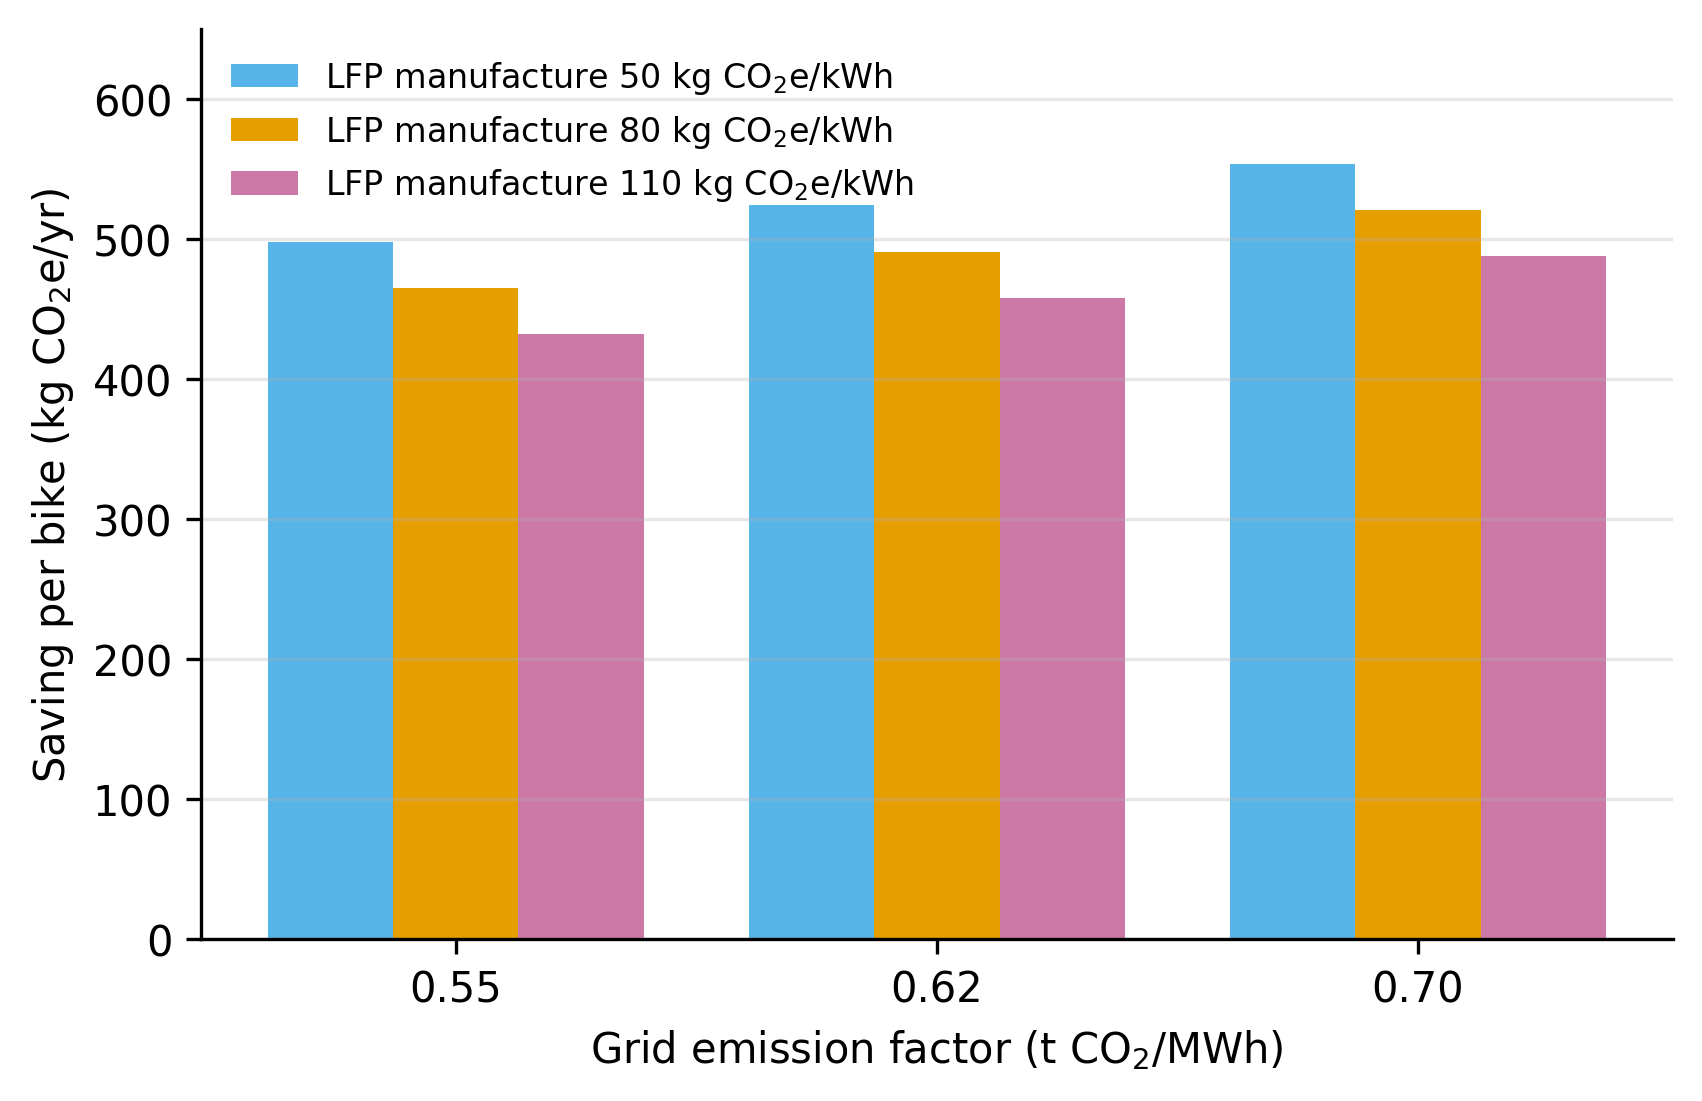
\includegraphics[width=.62\textwidth]{fig7_co2_sensitivity.png}\caption{Per-bike saving from LFP versus lead-acid for three LFP manufacturing footprints and three grid emission factors.}\label{fig:co2sens}\end{figure}

\subsection{Lead flow and policy scenarios}
\begin{table}[t]
\centering\small
\caption{Lead throughput of the lead-acid fleet (kt Pb per year through replacement and recycling). 125~kg is the figure published by Pure Earth \citep{pureearth_smep}; 60 and 90~kg are scenarios (battery mass $\times$ lead share).}
\label{tab:lead}
\begin{tabular}{lrr}
\toprule
Lead per pack & 1.4 M bikes & 3.0 M bikes \\
\midrule
60 kg & 82 & 175 \\
90 kg & 122 & 262 \\
125 kg & 170 & 364 \\
\bottomrule
\end{tabular}
\end{table}

\begin{table}[t]
\centering\small
\caption{Policy scenarios for a 1.4~M-bike fleet: share moved from lead-acid to LFP. Lead flow assumes 90~kg Pb per pack (60--125~kg, \cref{tab:lead}); savings are 10-year NPV to operators.}
\label{tab:policy}
\begin{tabular}{lrrrr}
\toprule
Scenario & LFP share & CO$_2$e saved & Pb cycled & Operator saving \\
 & (\%) & (Mt/yr) & (kt Pb/yr) & ($10^9$ BDT) \\
\midrule
S0 Business as usual & 0 & 0.00 & 122 & 0 \\
S1 Early adoption & 25 & 0.18 & 92 & 135 \\
S2 Targeted policy & 50 & 0.37 & 61 & 270 \\
S3 Full transition & 100 & 0.73 & 0 & 539 \\
\bottomrule
\end{tabular}
\end{table}

The lead-acid fleet cycles \leadLow--\leadHigh{}~kt of lead per year at 1.4~M bikes (\cref{tab:lead}); the upper value is close to the 167~kt reported by Pure Earth for the whole electric three-wheeler sector \citep{pureearth_smep}. Converted bikes need replacement so rarely that their lead flow in the model falls to zero. A 50\% conversion saves \polHalfCO{}~Mt\,CO$_2$e per year and BDT \polHalfSav{} billion for operators over ten years, and full conversion saves \polFullCO{}~Mt per year and BDT \polFullSav{} billion (\cref{tab:policy,fig:policy}).
\begin{figure}[t]\centering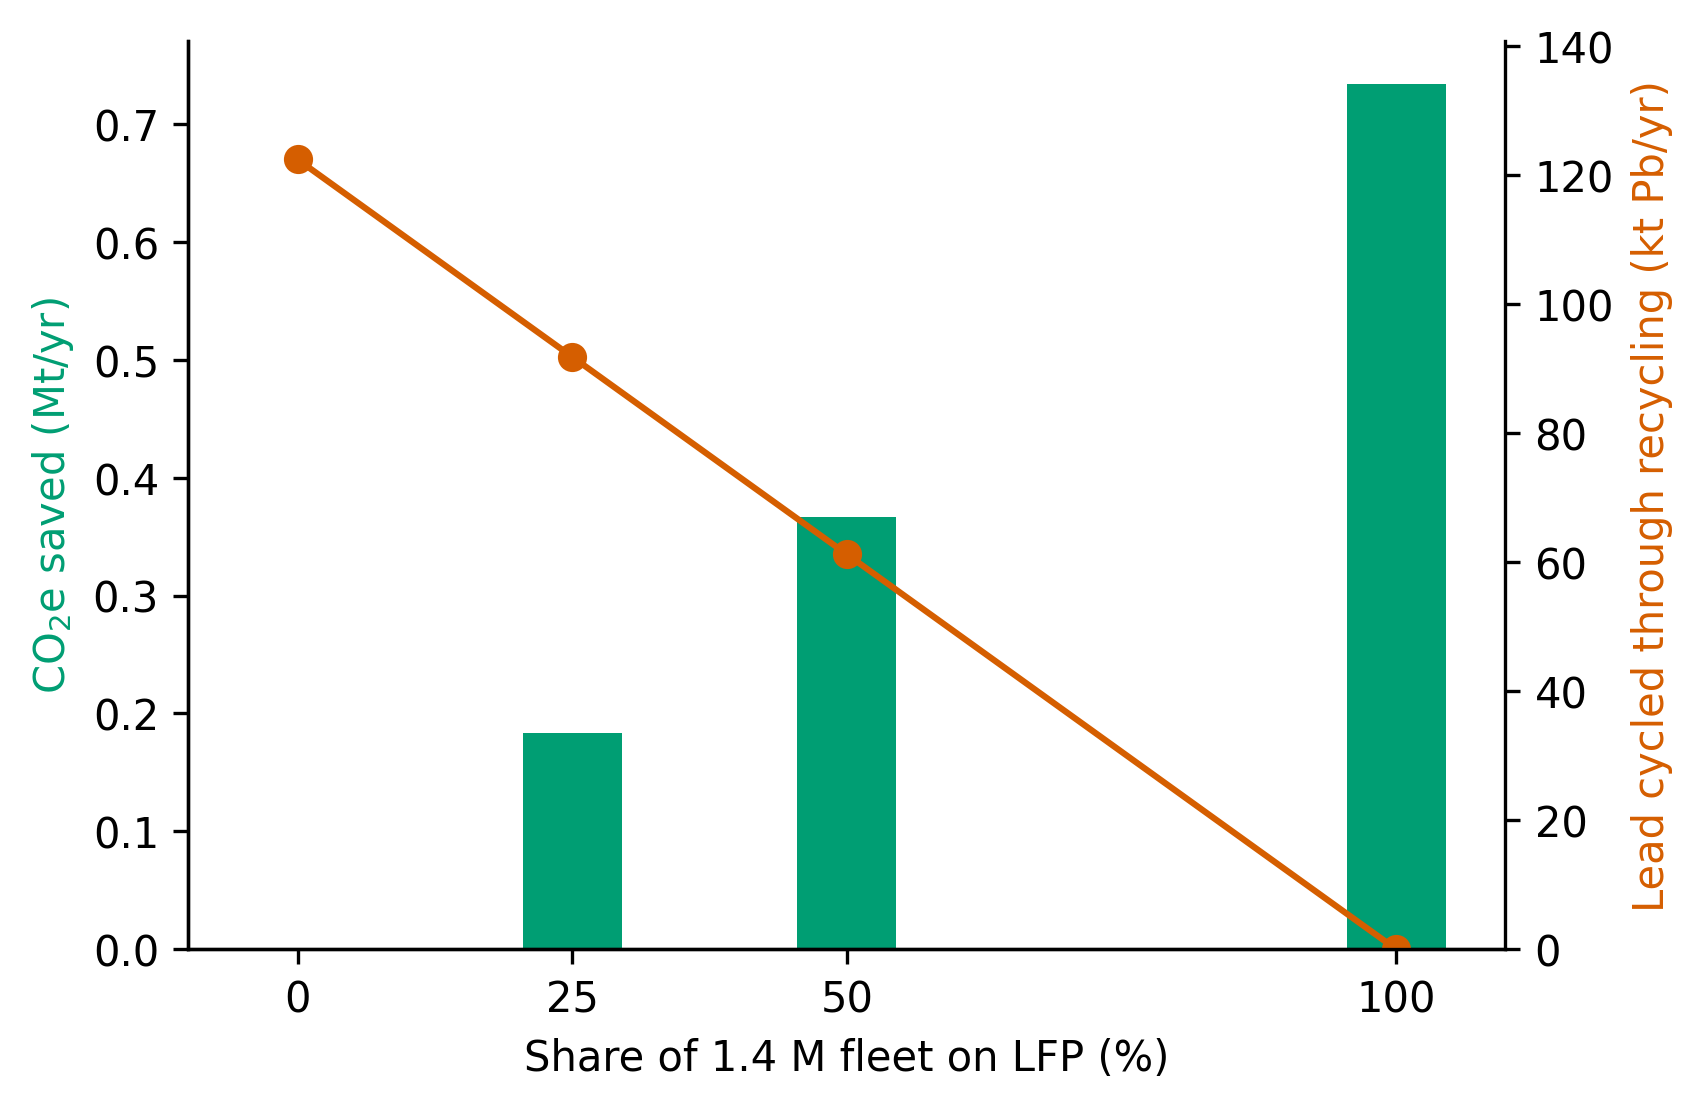
\includegraphics[width=.62\textwidth]{fig6_policy.png}\caption{Policy scenarios: CO$_2$e saved and lead cycled through recycling versus the share of the fleet on LFP.}\label{fig:policy}\end{figure}

\section{Discussion}
\subsection{Why LFP wins in this model}
Three mechanisms act together. First, LFP's higher round-trip efficiency cuts charging energy by \gridratio\%. Second, ageing at 30--34$^\circ$C is far slower per cycle for lithium, so one LFP pack outlasts about seven lead-acid packs. Third, fewer replacements mean fewer manufactured packs and less lead entering the recycling chain. The lead-acid life (\lifeLA{} months) is close to the 8--12 months reported in the field \citep{fe2024}, so the baseline is realistic; the LFP life of \lifeLFP{} months rests on laboratory-derived ageing laws and a cycle-life range, and has not been observed in Bangladeshi service, which is why operator data remain the most valuable next step. The ranking agrees with LCA findings that LFP is preferable where many daily cycles occur \citep{jasper2025,yudhistira2022}.

\subsection{Temperature: what matters and what does not}
Regional temperature does \emph{not} separate Khulna, Chuadanga and Rajshahi: mean battery temperatures differ by \Tspread$^\circ$C and every ranking is identical. Chemistry choice is therefore robust to site within the south-west. The temperature effect operates through the seasonal cycle, heat waves, and above all the battery's temperature rise above ambient (\cref{tab:scen}), the largest single uncertainty. Measuring pack temperature in service is a higher priority than adding weather stations.

\subsection{Carbon: a smaller prize than health, but robust}
A full switch saves about \fleetLFPa{}~Mt\,CO$_2$e per year at 1.4~M bikes, and the saving holds across manufacturing footprints of 50--110~kg\,CO$_2$e/kWh and grid factors of 0.55--0.70. As the grid decarbonises the operational saving falls while the embodied saving remains. The carbon case alone is not the strongest argument for switching; cost and lead are stronger.

\subsection{Lead, workers and public health}
Used lead-acid batteries are collected, broken open, and their lead plates smelted, often by hand and close to homes and farmland. Pure Earth describes informal recycling that contaminates and poisons workers and nearby residents \citep{pureearth_smep}; ESDO identifies it as a primary contributor to lead-pollution hotspots \citep{esdo2021}. The IEDCR bulletin reports that about 36~million children (60\%) are poisoned by lead, and that market screening in Dhaka, Rajshahi, Khulna and Barishal found 24\% of 197 consumer samples above reference lead levels; home assessments in 47 Khulna households found high lead in metal and ceramic cookware and toys \citep{das2026}. Children are most vulnerable: the World Health Organization notes that no safe level of lead exposure is known \citep{who_lead}. Remediation helps but only partly: soil lead fell 96\% at an abandoned Savar site while child blood lead fell 35\% \citep{chowdhury2021}; the IEDCR bulletin reports a 20\% fall at Mirzapur, where hotspot soil dropped from about 100{,}000 ppm to 60--100 ppm \citep{das2026}; and a Tangail study reports 22\% \citep{eos2026}. The fact that blood lead falls much less than soil lead suggests other sources persist, so removing the source of new contamination is as important as cleaning old sites. Between 70\% and 80\% of ULAB recycling is reported to be informal \citep{dailystar80,pureearth_smep,cpd2025}, and e-rickshaws and easy-bikes generate about 77\% of ULABs \citep{unep_ulab}.

Our model supplies the \emph{quantity} side: by extending battery life from about 12 to about 84~months, an LFP conversion removes \leadLow--\leadHigh{}~kt of lead per year from the recycling stream at 1.4~M bikes. It does not estimate how much of that lead would reach people; that needs emission and exposure data that do not yet exist, and other sources (paint, spices, cookware) also contribute. \begin{figure}[t]\centering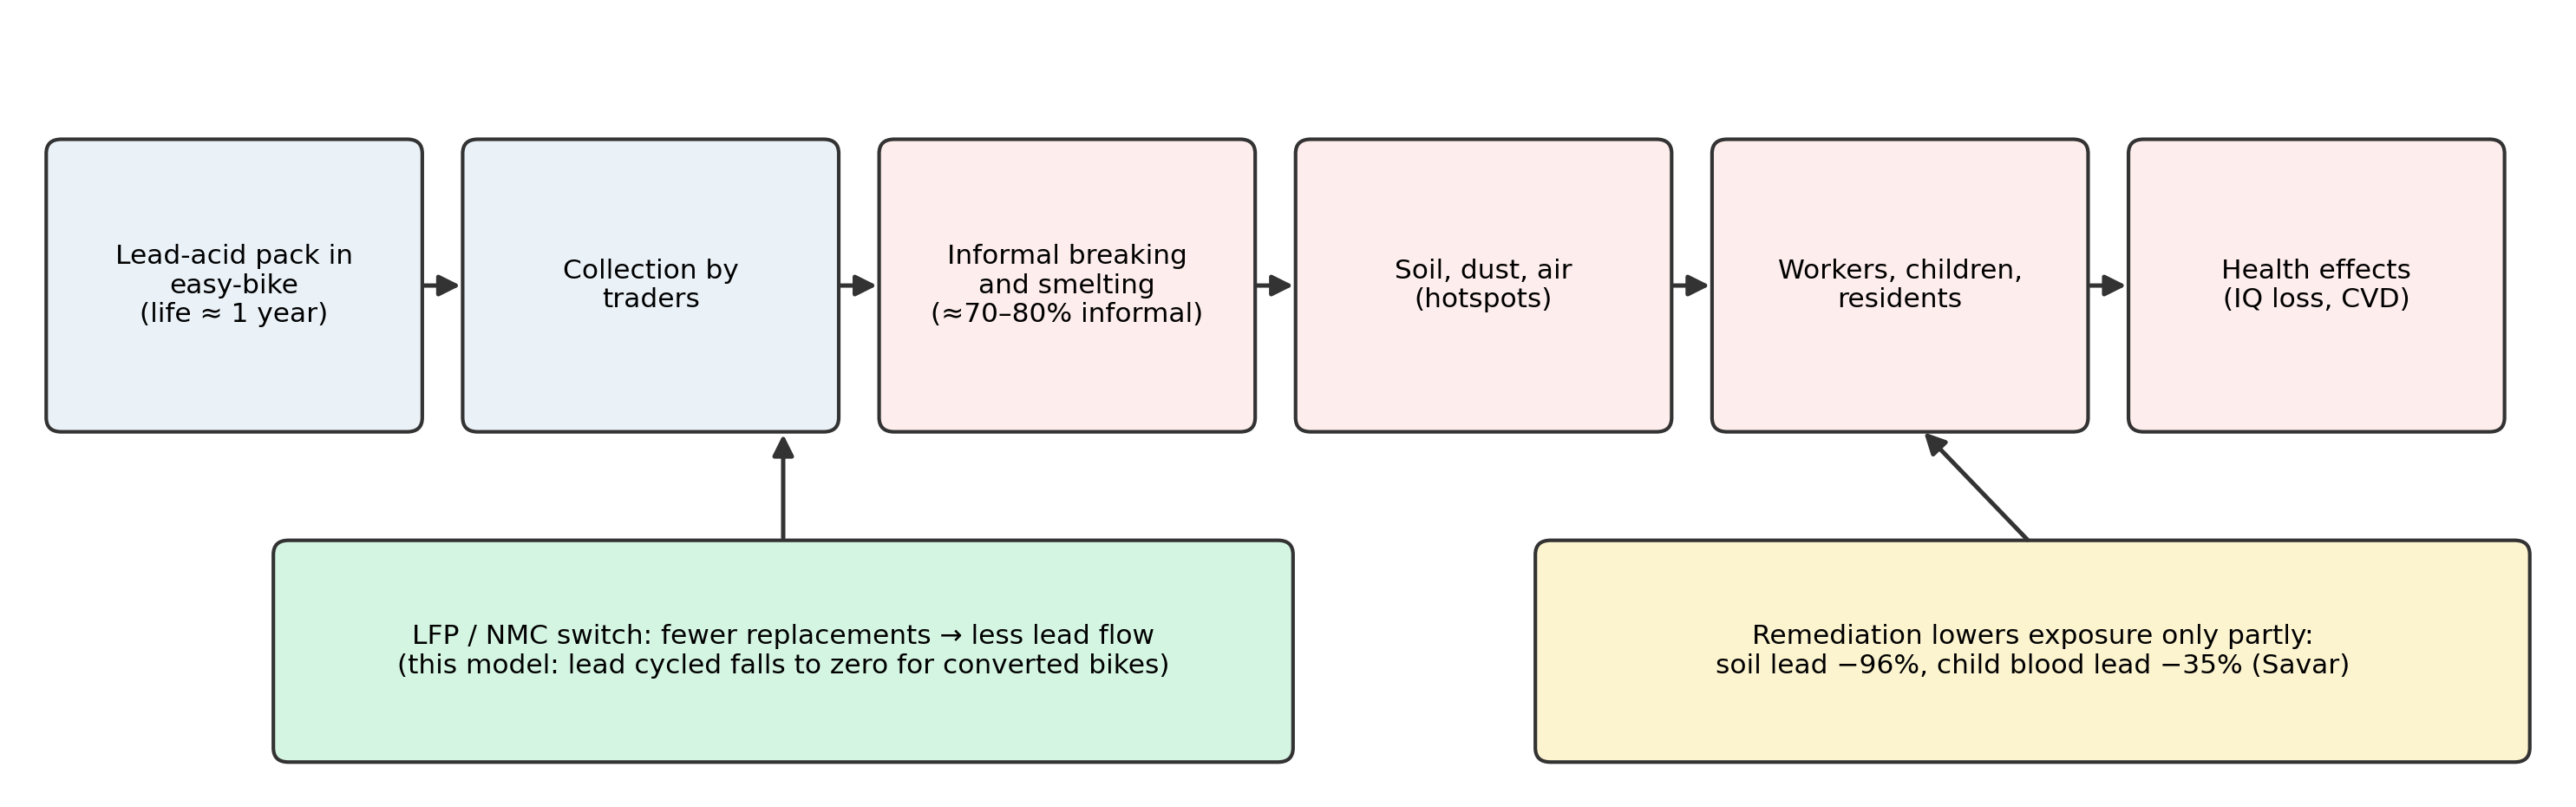
\includegraphics[width=\textwidth]{fig_lead.png}\caption{Pathway from lead-acid easy-bike batteries to exposure (schematic) and the point where an LFP switch acts; remediation figures from \citep{chowdhury2021}.}\label{fig:lead}\end{figure}

\subsection{Policy implications}
(i)~\emph{Up-front finance}: the BDT \premium{} premium is repaid in about \paybackYr{} year, so the barrier is capital access, not total cost; pay-as-you-go and battery-swap schemes address this \citep{smep2024}. (ii)~\emph{Taxes and duties}: current taxes on lithium batteries are described as unfavourable \citep{smep2024}, while the break-even price of about BDT \beLFP{} leaves large room for relief. (iii)~\emph{ULAB regulation}: the 2021 Hazardous Waste (e-waste) Management Rules reportedly cover household but not e-rickshaw lead batteries \citep{smep2024}. (iv)~\emph{Lithium end-of-life}: a collection and recycling route must exist before volumes grow.

\subsection{Limitations}\label{sec:limits}
\begin{itemize}[nosep]
\item \textbf{No operator records.} Battery temperature rise, operating days and scrap value are scenarios; daily distance is calibrated to a published energy per charge. The model is plausible against published ranges but not validated against operator data.
\item \textbf{Cycle-limited life.} Calendar ageing is not modelled; the LFP life of \lifeLFP{} months (about 7 years) may be optimistic in hot, rough service, though the 10-year cost includes only one replacement.
\item \textbf{Vendor-level capacity curves} for the temperature dependence of capacity; the effect is small between 20 and 45$^\circ$C.
\item \textbf{Monthly temperature.} Hourly data would capture daily peaks and charging-time heat.
\item \textbf{Single-site field study.} Duty inputs come from one instrumented bike and a survey in Gopalganj and Khulna \citep{chowdhury2026}.
\item \textbf{Fleet size.} 1.4~M and 3--4~M are both reported; results scale linearly.
\item \textbf{Weight, fire safety and imports} are not modelled.
\item \textbf{Lead flow is not exposure.}
\item \textbf{Tariff.} The BDT 11.36/kWh rate is from the June 2026 order as reported by the press; wholesale prices were revised again in August 2026 \citep{observer2026}. Tariffs of 7.70--16.24 change the cost gap by less than 3\% (\cref{tab:scen}).
\end{itemize}

\section{Conclusion}
Using published data and a transparent, reproducible model, LFP batteries outperform lead-acid for Bangladesh easy-bikes on efficiency (\effLFP{} vs \effLA\%), life (about \lifeLFP{} vs \lifeLA{} months), 10-year cost (BDT \tcoLFP{} vs \tcoLA) and carbon (about \saveLFPbike{}~kg\,CO$_2$e per bike-year). NMC lies between the two. The ranking is the same at Khulna, Chuadanga and Rajshahi, so site temperature does not change it, while battery heating and heat waves widen the lead-acid disadvantage. A full switch of a 1.4~M fleet would save about \fleetLFPa{}~Mt\,CO$_2$e per year and remove \leadLow--\leadHigh{}~kt of lead per year from informal recycling. The premium is repaid in about a year, pointing policy toward financing, taxes and recycling rules. LFP's cost advantage is robust to any single input but can disappear when several unfavourable assumptions combine; operator records on distance, pack temperature and scrap value are the priority for confirming it.
\section{Reproducibility}
Run in MATLAB R2024a: (1) \texttt{easybike\_main} (tables and figures); (2) \texttt{easybike\_co2} (carbon, lead and policy); (3) \texttt{easybike\_build\_simulink} (Simulink verification; needs Simulink); (4) \texttt{easybike\_check} (compares your \texttt{results\_summary.csv} with the values in this paper). Inputs live in \texttt{easybike\_params.m}, each tagged with its source key. NASA POWER files: Monthly, T2M, 2024-01-01 to 2025-12-31, local solar time, points 22.84$^\circ$N 89.57$^\circ$E, 23.64$^\circ$N 88.69$^\circ$E and 24.38$^\circ$N 88.60$^\circ$E. Tables and figures in this paper were generated by a Python port that reproduced a previous MATLAB \texttt{results\_summary.csv} to 15 significant digits; the MATLAB code in the final form must be run once to confirm Tables 4--8.

\section*{Declarations}
\noindent\textbf{Data availability.} NASA POWER files, MATLAB/Simulink code (\texttt{easybike\_*.m}, \texttt{easybike\_battery.slx}) and all result tables are provided as supplementary material. \todo{deposit on Zenodo/GitHub and add DOI}\\
\textbf{Funding / Conflicts of interest.} \todo{complete}\\
\textbf{Acknowledgements.} \todo{complete}
\bibliographystyle{unsrtnat}
\bibliography{references}
\appendix
\section{Data and parameter files}
\texttt{matlab/expected\_results.csv} holds the nine site-battery rows behind \cref{tab:results}. \texttt{easybike\_check.m} reports whether your MATLAB output matches them.

\end{document}
